%% Copernicus Publications Manuscript Preparation Template for LaTeX Submissions
%% ---------------------------------
%% This template should be used for copernicus.cls
%% The class file and some style files are bundled in the Copernicus Latex Package, which can be downloaded from the different journal webpages.
%% For further assistance please contact Copernicus Publications at: production@copernicus.org
%% https://publications.copernicus.org/for_authors/manuscript_preparation.html


%% Please use the following documentclass and journal abbreviations for preprints and final revised papers.
%% Development and technical papers
%% 2-column papers and preprints
\documentclass[journal abbreviation, manuscript]{copernicus}



%% Journal abbreviations (please use the same for preprints and final revised papers)


% Advances in Geosciences (adgeo)
% Advances in Radio Science (ars)
% Advances in Science and Research (asr)
% Advances in Statistical Climatology, Meteorology and Oceanography (ascmo)
% Annales Geophysicae (angeo)
% Archives Animal Breeding (aab)
% Atmospheric Chemistry and Physics (acp)
% Atmospheric Measurement Techniques (amt)
% Biogeosciences (bg)
% Climate of the Past (cp)
% DEUQUA Special Publications (deuquasp)
% Drinking Water Engineering and Science (dwes)
% Earth Surface Dynamics (esurf)
% Earth System Dynamics (esd)
% Earth System Science Data (essd)
% E&G Quaternary Science Journal (egqsj)
% EGUsphere (egusphere) | This is only for EGUsphere preprints submitted without relation to an EGU journal.
% European Journal of Mineralogy (ejm)
% Fossil Record (fr)
% Geochronology (gchron)
% Geographica Helvetica (gh)
% Geoscience Communication (gc)
% Geoscientific Instrumentation, Methods and Data Systems (gi)
% Geoscientific Model Development (gmd)
% History of Geo- and Space Sciences (hgss)
% Hydrology and Earth System Sciences (hess)
% Journal of Bone and Joint Infection (jbji)
% Journal of Micropalaeontology (jm)
% Journal of Sensors and Sensor Systems (jsss)
% Magnetic Resonance (mr)
% Mechanical Sciences (ms)
% Natural Hazards and Earth System Sciences (nhess)
% Nonlinear Processes in Geophysics (npg)
% Ocean Science (os)
% Polarforschung - Journal of the German Society for Polar Research (polf)
% Primate Biology (pb)
% Proceedings of the International Association of Hydrological Sciences (piahs)
% Safety of Nuclear Waste Disposal (sand)
% Scientific Drilling (sd)
% SOIL (soil)
% Solid Earth (se)
% State of the Planet (sp)
% The Cryosphere (tc)
% Weather and Climate Dynamics (wcd)
% Web Ecology (we)
% Wind Energy Science (wes)


%% \usepackage commands included in the copernicus.cls:
%\usepackage[german, english]{babel}
%\usepackage{tabularx}
%\usepackage{cancel}
%\usepackage{multirow}
%\usepackage{supertabular}
%\usepackage{algorithmic}
%\usepackage{algorithm}
%\usepackage{amsthm}
%\usepackage{float}
%\usepackage{subfig}
%\usepackage{rotating}


\begin{document}

\title{Impacts of spatial heterogeneity of anthropogenic aerosol emissions in a high-resolution Earth system model
}


% \Author[affil]{given_name}{surname}

\Author[1]{Taufiq}{Hassan}
\Author[1]{Kai}{Zhang}
\Author[1]{Jianfeng}{Li}
\Author[1]{Balwinder}{Singh}
\Author[1]{Shixuan}{Zhang}
\Author[1]{Hailong}{Wang}
\Author[1]{Po-Lun}{Ma}

\affil[1]{Atmospheric Sciences and Global Change Division, Pacific Northwest National Laboratory, Richland, WA, USA}

%% The [] brackets identify the author with the corresponding affiliation. 1, 2, 3, etc. should be inserted.

%% If an author is deceased, please mark the respective author name(s) with a dagger, e.g. "\Author[2,$\dag$]{Anton}{Smith}", and add a further "\affil[$\dag$]{deceased, 1 July 2019}".

%% If authors contributed equally, please mark the respective author names with an asterisk, e.g. "\Author[2,*]{Anton}{Smith}" and "\Author[3,*]{Bradley}{Miller}" and add a further affiliation: "\affil[*]{These authors contributed equally to this work.}".


\correspondence{Taufiq Hassan (taufiq.hassan@pnnl.gov) and Kai Zhang (kai.zhang@pnnl.gov)}

\runningtitle{TEXT}

\runningauthor{TEXT}





\received{}
\pubdiscuss{} %% only important for two-stage journals
\revised{}
\accepted{}
\published{}

%% These dates will be inserted by Copernicus Publications during the typesetting process.


\firstpage{1}

\maketitle



%\begin{abstract}
%TEXT
%\end{abstract}

\begin{abstract}
Emissions of anthropogenic aerosol particles and their precursors are often prescribed in global aerosol models. Most of these emissions are spatially heterogeneous at model grid scales. When remapped from low-resolution data, the spatial heterogeneity in emissions can be lost, leading to large errors in the simulation. It can also cause the conservation problem if non-conservative remapping is used. The default emission treatment in Energy Exascale Earth System Model (E3SM) suffers from both problems. In this study, we introduce a new emission treatment for the E3SM atmosphere model (EAM) that ensures conservation of mass fluxes and preserves the original emission heterogeneity. We assess the error estimates associated with the default emission treatment and the impact of resolved heterogeneity and mass conservation in both globally uniform standard-resolution ($\sim$100 km) and regionally refined high-resolution (< 50 km) simulations. The default treatment incurs significant errors near surface, particularly over sharp emission gradient zones, with larger errors in high-resolution simulations. The default treatment significantly underestimates (overestimates) aerosol burden, surface concentration, aerosol sources (aerosol sinks) over highly polluted regions, while overestimating (underestimating) them over nearby less polluted regions. Large errors can persist at higher elevation from daily mean estimates, which can affect aerosol extinction profiles and aerosol optical depth (AOD). Our new treatment significantly improves the accuracy of the aerosol emissions from surface and elevated sources near sharp spatial gradient regions, with significant improvement in the spatial heterogeneity and variability of simulated surface concentration in high-resolution simulations. We utilized routines to assimilate emissions at the model-native Spectral Element (SE) grid, making it suitable for any resolution and applicable to both uniform resolution and Regionally Refined Model (RRM) configurations. Our findings suggest the new emission treatment is crucial for future E3SM applications with regional refinement at high resolutions, such as convection-permitting scales, to help improve the simulated aerosol lifecycle and the aerosol impact on climate.
\end{abstract}

%\copyrightstatement{TEXT} %% This section is optional and can be used for copyright transfers.


%\introduction  %% \introduction[modified heading if necessary]
%TEXT
\section{Introduction}

The presence of lower tropospheric aerosols has significant impacts on air quality and human health. Studies have shown that aggravated aerosol pollution in terms of fine particulate matter (PM2.5), contributes to over a million premature deaths annually \citep{lelieveld2015contribution,davidson2005airborne}. Additionally, aerosols play a crucial role in the energy balance of the Earth system, as they can scatter or absorb radiation and indirectly affect the formation, lifetime, and albedo of clouds. Anthropogenic activities, including human-made pollution, have contributed to a substantial increase in the tropospheric aerosol burden since the pre-industrial era, further intensifying these effects \citep{Bond07}. According to the report on the 6th Intergovernmental Panel on Climate Change (IPCC), the anthropogenic aerosol effective aerosol radiative forcing ranges from -0.63 to -1.37 W m-2 \citep{smith2020effective}. Furthermore, recent urban-scale studies have shown that anthropogenic aerosols may impact regional climate by affecting the urban heat island intensity \citep{han2020mechanisms,yang2020pm2,wu2017urban} and altering the precipitating systems over urban areas \citep{rosenfeld2008flood,van2007urban}. Despite the crucial role of anthropogenic aerosols in regional and global climate, significant uncertainties persist in their numerical simulation. This uncertainty is due to a limited understanding regarding their emissions, distribution in the atmosphere, and optical properties \citep{kinne2006aerocom,schulz2006radiative,textor2006analysis,myhre2013radiative,samset2013black}.

The accurate representation of anthropogenic aerosol emissions and their consistent time series data are crucial for Earth system models (ESMs) and atmospheric chemistry and transport models \citep{hoesly2018historical}. The prescribed emission time series serve as key inputs to these models, which use recent aerosol emissions as a starting point to predict future aerosol concentrations. However, most of these emission sources are spatially heterogeneous at regional and local scales, and their relatively short lifetime in the atmosphere results in a heterogeneous distribution, both geographically and vertically \citep{koch2009evaluation}. Retaining this heterogeneity during simulations is critical since model performance evaluation in areas such as aerosol formation, transport, cloud interactions, and deposition depends on the quality of the prescribed emissions used to drive the models. Using lower-resolution data may result in a loss of heterogeneity, leading to lower accuracy in the aerosol simulation and model evaluations, particularly near the sharp emission gradient zones. This error may be more significant for high-resolution model simulations, often used in urban-scale studies.

The U.S. Department of Energy (DOE) Energy Exascale Earth System Model (E3SM) is a state-of-the-art ESM that aims to produce actionable and accurate predictions of regional trends relevant to Earth system variability and change \citep{golaz2019doe}. The E3SM atmosphere model (EAM) has several parameterizations to represent different physical and chemical processes, including an aerosol emission treatment to handle prescribed emissions, which can impact the horizontal and vertical distribution of simulated aerosol concentration, their lifecycle, and interactions with clouds and radiation \citep{burrows2022oceanfilms,liu2012toward,liu2016description,wang2020aerosols}. However, the default emission treatment used in the standard and high-resolution EAM configurations has some limitations. Like many atmospheric models, EAM uses an unstructured cubed-sphere spectral-element (SE) grid due to its advantages over regular latitude-longitude (RLL) grids, such as offering high-resolution capabilities and improved computational scalability through Regionally Refined Mesh (RRM) \citep{taylor2010compatible,dennis2012cam}. Since conservative regridding within E3SM is not currently available, EAM linearly interpolates input emissions data to the model-native SE grid, which leads to a lack of mass conservation in current E3SM simulations. Furthermore, for low-resolution and RRM simulations, EAM uses low-resolution ($\sim$2$^{\circ}$) anthropogenic aerosol emission data, which fails to preserve the spatial heterogeneity in prescribed emissions. Therefore, improving the emission treatment in EAM is essential, especially for future E3SM applications with regional refinement at high resolutions, such as convection-permitting scales.

In this study, we introduce a new emission treatment for the Energy Exascale Earth System Model (E3SM) that ensures conservation of mass fluxes and preserves the original emission heterogeneity. Our objective is to assess the error estimates associated with the default emission treatment and the impact of resolved heterogeneity and mass conservation in high-resolution simulations. Our new treatment approach utilizes routines to assimilate emissions at the model-native Spectral Element (SE) grid, which makes it suitable for any resolution and applicable to both uniform resolution and Regionally Refined Mesh (RRM) configurations. This new treatment is crucial for implementing accurate emissions in future aerosol model evaluations at high-resolution urban to convection-permitting scale. 

This article is organized as follows: In Section 2, we provide a detailed account of the methods used, including the model configuration and experimental setups. In Section 3, we present the results of our study, including improved anthropogenic aerosol emission data, model comparison results, and an evaluation of our model against observations. Finally, we summarize our findings and provide conclusions in Section 4.


\section{Methods}
In this section, we provide description of the model used for this study, process of implementing the new emission treatment in the model, and the experimental design to evaluate the new treatment.

\subsection{Model Configuration}
In this study, we utilize the atmosphere component (EAMv2) of the Energy Exascale Earth System Model version 2 (E3SMv2) \citep{golaz2022doe}, which was developed by the United States Department of Energy (DoE), to investigate the impact of the new emission treatment on aerosol processes. E3SMv2 includes a comprehensive aerosol model, derived from the four-mode version of Modal Aerosol Module (MAM4), representing major anthropogenic and natural aerosol species, including black carbon (BC), primary organic matter (POM), secondary organic aerosol (SOA), marine organic aerosol (MOA), sulfate, mineral dust, and sea-salt in four lognormal size modes \citep{wang2020aerosols,liu2016description}. The model accounts for various aerosol processes including nucleation, coagulation, condensation, SOA formation, convective transport, wet removal, and dry deposition.

EAMv2 employs a spectral element dynamical core as in EAMv1 \citep{taylor2010compatible,dennis2012cam}, but utilizes “physics grid” (pg2 grid) for unresolved physics parameterization and a separate dynamics grid for resolved processes. This allows for an increased computational efficiency by reducing the effective resolution for the physics parameterization computations. The standard configuration of the model uses a low “ne30pg2” resolution (LR), which has a grid spacing of $\sim$110 km ($\sim$1$^{\circ}$) for dynamics and a grid spacing of $\sim$165 km ($\sim$1.5$^{\circ}$) for physics. E3SMv2 also supports fully coupled regionally refined mesh (RRM) configurations for high-resolution applications. One of the supported stable RRM configurations has a high-resolution mesh centered over North America (NA RRM). The NA RRM setup has a horizontal resolution of ne120pg2 ($\sim$28-km dynamics grid and $\sim$42-km physics grid) over North America and a horizontal resolution of ne30pg2 over rest of the globe (Fig. 1b). The high-resolution refined mesh is located approximately within 10$^{\circ}$N to 80$^{\circ}$N and 170$^{\circ}$W to 10$^{\circ}$W. This region covers a significant number of observation sites (AERONET and IMPROVE) for model evaluation (Fig. 1a). NA RRM has a total of 57816 computational elements or grid cells as opposed to 21600 in the standard configuration.

In the present study, we conduct experiments in both LR and NA RRM setup to explore the impact of the new emission treatment. More detailed description of the experimental setups is available in section 2.4.

\subsection{E3SM emission treatment}

The original source of anthropogenic emissions from agricultural, industrial, energy, transportation, and domestic sectors for EAMv2 are mostly derived from Community Emissions Data System (CEDS) inventory \citep{hoesly2018historical}. The biomass burning emission is derived from the fourth generation of the Global Fire Emissions Database (GFED4) \citep{giglio2013analysis,van2017historic}. CEDS provides historical (1750$-$2014) inventory of anthropogenic GHGs, reactive gases, and aerosols for Coupled Model Intercomparison Project phase 6 (CMIP6) \citep{eyring2016overview}. It includes anthropogenic emissions for the primary aerosol species, such as black carbon (BC) and organic carbon (OC), and chemically reactive gas sulfur-di-oxide (SO$_2$) as a precursor for Sulfate aerosols (SO$_4$). These data are in regular latitude longitude (RLL) grid at {0.5}$^{\circ}$\times{0.5}$^{\circ}$ resolution. GFED4 is also a part of the inputs for CMIP6, which provides historical (1750$-$2015) anthropogenic aerosol emission inventory of BC, OC, and SO$_2$ from biomass burning in RLL grid at {0.25}$^{\circ}$\times{0.25}$^{\circ}$ resolution. In the standard configuration of EAMv2, low resolution ({1.9}$^{\circ}$\times{2.5}$^{\circ}$) RLL gridded monthly historical (1850-2014) emission data are prescribed for ne30pg2 and RRM simulations. EAM also considers vertically distributed emissions from biomass burning, industrial, energy, and volcanic sources. These elevated emissions are distributed across 13 different altitudes, ranging from the ground level to approximately 7 km above the surface. The distribution of emission within each layer is uniform, but the distribution varies between layers, depending on the source of the emission. Elevated sulfur emissions from energy and industrial sectors are emitted at altitudes between 100 and 300 meters above the surface, while biomass burning emissions are distributed across all 13 altitude ranges, with diminishing fractions at higher elevations.

The emission treatment is a key component of the post-coupler processes. The EAMv2 utilizes consistent routines to process all prescribed anthropogenic aerosol and precursor gas emissions, where they are read from regular latitude-longitude gridded inputs, initialized either as emission fluxes or elevated sources, and are subsequently spatiotemporally interpolated to account for the model-native spectral element (SE) grid compatibility. The interpolated emission data are passed to the aerosol microphysics modules. The aerosol microphysics modules simulate the formation, growth, and removal of aerosols in the atmosphere, including processes of nucleation, coagulation, condensation, and sedimentation. During this stage, the elevated emissions are applied to the gas-phase chemistry calculations, and the surface fluxes are updated before dry deposition estimates are made (Fig. 2a).

EAMv2 considers emissions at the bottom layer of the model as surface emission fluxes and vertically distributed emissions as elevated sources. So, surface layer emissions and vertically injected emissions are handled separately (Fig. 2b). However, EAMv2 treats anthropogenic emissions and prescribed natural emissions (e.g., Dimethyl sulfate (DMS) ) in the same manner, and all computations are performed on the  model-native grid. The original EAMv2  can not handle emission data on  the model-native SE grid. Since all available emissions data sources are provided in RLL grid format, interpolation is needed to regrid the data into model-native grid structure. After the spatial interpolation, the model also performs temporal interpolation. In EAMv2, linear interpolation is applied to convert the prescribed RLL grid data to model-native grid. Although it’s convenient to linearly interpolate the same emission data to model grid at different spatial resolutions, the current treatment does not conserve mass. Also, when interpolated to higher resolutions, large emission errors will occur compared to the original emission data.

\subsection{New emission treatment}

To address the limitations of the default emission treatment in E3SM, we implemented a new emission treatment. The new treatment modifies the current treatment in the following ways:
\begin{enumerate}
\item	We have modified aerosol emission routines, which allows EAM to read prescribed anthropogenic aerosol emissions in both regular latitude-longitude (RLL) and model-native (SE) grids.
\item	To preserve spatial heterogeneity and mass conservation, we prepare the emission data on model-native grids offline using a conservative remapping tool using a high-resolution emission inventory as input. The online linear interpolation is switched off when the new treatment is used (reading the conservatively remapped data directly. 
\end{enumerate}
The new treatment has been implemented in both EAMv1 and EAMv2 for scientific evaluations. To simplify and automate the offline steps (Fig. 2b), we developed a Python wrapper package that utilizes TempestRemap \citep{ullrich2015arbitrary,ullrich2016arbitrary} and ncremap \citep{zender2008analysis}. This complementary grid generator tool (ggen) is used to generate grids, weights, and re-format the high-resolution emission data to the new emission treatment compatible format in model-native grid. This package is applicable to both surface and elevated emissions at any resolution.  

In this study, we use {0.63}$^{\circ}$\times{0.47}$^{\circ}$ RLL grid anthropogenic aerosol and precursor gas emission data as the high-resolution emission source, which were derived from the original CEDS and GFEDv4 data set and retains the injection heights for the vertically distributed emissions as in the default treatment. However, this new treatment can also be applied to other emissions data at any resolutions in RLL, model-native, and RRM grid formats. As will be shown later, the new treatment significantly improves the emission spatial heterogeneity in high-resolution applications.

\subsection{Experimental setup}

Two groups of E3SMv2 simulations at different horizontal resolutions were conducted to estimate the impacts of the new emission treatment in EAMv2 (Table 1).  Each group consists of control simulations using the default emission treatment and spectral-element (SE) treatment simulations utilizing the new emission treatment. The simulations were performed for both the low-resolution standard configuration of E3SMv2 (ne30pg2 or LR) and high-resolution (NA RRM) setup with 72 vertical layers (Fig. 1). For the control simulations, we follow the standard configuration and use the default low-resolution (1.9x2.5$^{\circ}$) prescribed emissions of aerosols and precursor gases in RLL grid. For SE simulations, we prepared anthropogenic aerosols and precursor gas emission on model-native grid from a high-resolution inventory. We conducted simulations with both Present-Day (PD, year 2014) anthropogenic aerosol emissions, and Pre-Industrial (PI, year 1850) anthropogenic aerosol emissions. All simulations include active atmosphere and land with prescribed monthly mean climatological SST and sea ice from 2005-2014.

All simulations were conducted using a meteorological nudging method \citep{sun2019impact,zhang2022further}, in which the horizontal wind components (u and v) were nudged to the European Centre for Medium-Range Weather Forecasts (ECMWF) ERA5 reanalysis \citep{hersbach2020era5}. These simulations were performed from October 1st, 2015, to December 31st, 2016. The first three months from the year 2015 were discarded as a model spin-up period, and the remaining 12 months were used for the analysis in this study. To perform these nudging simulations in EAMv2 at both LR and RRM resolutions, ERA5 reanalysis data from the year 2015-2016 were prepared for EAMv2 spectral-element (SE) dynamical core. These data in SE grid were used to nudge the simulation meteorology, using a relaxation timescale of 6 hours.

\subsection{Observation Data}

To evaluate the model's ability to simulate regional to local aerosols with the updated emission treatment, simulated values for the surface concentrations of Black Carbon (BC), Primary Organic Matter (POM), and Sulfate (SO$_4$) aerosols, and optical properties such as Aerosol Optical Depth (AOD) are compared to observational data from regional networks such as the Interagency Monitoring of PROtected Visual Environment (IMPROVE) and Aerosol Robotic NETwork (AERONET) (Fig. 1a). Only present-day (PD) simulations (LR-PD and RRM-PD) were used for the evaluations.

IMPROVE, is a network of aerosol monitoring stations located in protected areas in the United States, such as national parks and wilderness areas \citep{malm2004spatial}. This network measures aerosol properties such as surface concentrations, size distribution, composition, and optical properties. IMPROVE surface concentration measurements are only available over the United States and provide daily data 3 times a week. For this evaluation, we consider daily average surface concentration measurements from all available IMPROVE sites for each aerosol species in the year 2016. Measurements are available from over 150 sites for BC, organic carbon (OC), and sulfate aerosol surface concentration. We also multiply the observed OC by 1.4 before comparing against simulated POM. Since the IMPROVE measurements are for fine aerosol particles, we do not consider simulated aerosols in coarse mode. We also applied a conversion factor of 96/115 ($\sim$0.83) to the simulated sulfate concentration before comparing against the IMPROVE measurements.

AERONET, on the other hand, a global network of ground-based sunphotometers, measures aerosol properties such as size distribution, composition, and optical properties \citep{holben1998aeronet}. For this evaluation, we used AOD spectral radiometer daily mean measurements from over 120 active sites during the simulation year (e.g., 2016), which fall within the North America high-resolution mesh (bounded by 15$^{\circ}$N to 75$^{\circ}$N and 55$^{\circ}$W to 170$^{\circ}$W) in the RRM setup. 

The simulated daily mean data were spatiotemporally aligned with the observational data according to the time and location of each active observational site. These daily average data were conditionally sampled based on EAMv2 emission differences found between the default and new treatment (see details in section 3.3). We consider the same sites for RRM and LR simulation evaluations. Finally, monthly mean of these spatiotemporally collocated data were used to compare simulated and observed surface concentration and AOD.




%\section{HEADING}
%TEXT
\section{Results and Discussions}

\subsection{Improving emissions in EAM}

One of the primary goals of our new emission treatment is to enhance the accuracy of the emissions data utilized in the standard LR and RRM simulations. The default EAM emissions treatment fails to preserve spatial heterogeneity or conserve mass, resulting in substantial errors (as described in section 2.2). Figure 3 illustrates the spatial distribution of total emitted surface Black Carbon (BC) and SO$_2$ over the Eastern United States in 2014. Column integrated SO$_2$, the primary precursor to Sulfate aerosols, depicts the spatial distribution of elevated sources in EAMv2. Figure 3 indicates how well the heterogeneity of prescribed surface and elevated emissions are represented in the standard RRM simulations when compared against the original high-resolution data.

The original high-resolution data display highly heterogeneous emissions over the land surface, largely driven by industrial, energy, and transportation sectors (Figure 3a, d). As expected, the default emission treatment fails to capture much of the heterogeneity over sharp emission gradient zones (Figure 3b, e). For example, panel b and e depict seven major cities (e.g., Boston, New York, Chicago, Toronto, Montreal, Los Angeles, and San Francisco) with large anthropogenic BC and SO$_2$ emissions respectively. The default treatment not only significantly underestimates emissions ($\sim$80\%) from those cities, but also grossly misrepresents emissions in the nearby regions. This can severely impact the accuracy of high-resolution studies over urban regions. Additionally, the default treatment provides an inaccurate representation of emissions near the coasts, where regions of BC sources from shipping sectors are misrepresented by comparatively large emissions from transport and industrial sectors. In general, both surface and vertically distributed emissions in the default treatment fail to maintain emission land-sea contrast near the coastlines. In contrast, panels c and f illustrate the spatial emissions distributions in the improved treatment, which accurately preserves the original spatial heterogeneity both inland and near the coast. Supplementary Fig. S1 depicts the large error regions in terms of the emission difference between the improved and default treatment from surface and elevated sources. It also indicates that larger errors, from sharper spatial gradients, exist near regions with larger emission. For instance, the difference from surface BC and POM is much larger over the Eastern US, which is consistent with the larger surface emissions over the Eastern US. This is important to separate the regions with sharper spatial gradients in the later sections. These improved datasets, which retain both heterogeneity and mass conservation, provide a more accurate representation of surface and vertically distributed emissions in EAMv2. It also accurately applies prescribed emissions in major cities, making the new treatment suitable for urban-scale studies.

To evaluate the loss of accuracy of the EAMv2 emissions in the default treatment, we calculate error estimates against more accurate emissions data, which preserve the original spatial heterogeneity and mass conservation. Table 2 provides a summary of the error estimates for Black Carbon (BC), Primary Organic Matter (POM), and Sulfate (SO$_4$) aerosol emissions data used in the EAMv2 RRM simulations, including area-weighted spatial mean (Mean), normalized mean bias (NMB), standard deviation (StdDev), normalized standard deviation (NStdDevB), root mean square error (RMSE), and normalized RMSE (N\_RMSE) for the present-day (year 2014). The values for elevated sources are estimated over column integrated spatial distributions. Table S1 presents the error statistics for emissions in the LR simulations. The RRM configuration in this study has a high-resolution mesh over North America (NA), with the largest sources of emissions occurring over the land and only emissions from the shipping sector occurring over the ocean. Therefore, we consider NA land surfaces bounded by 15N to 75N and 55W to 170W for the error estimates.

Our results indicate that the default treatment for anthropogenic aerosol emissions in both LR and RRM simulations consistently yields large root mean square errors (RMSE) for all species. It is worth noting that the normalized mean bias (NMB), which indicates mass conservation errors, is generally small (< 1\%) for long-term global estimates. However, it can be considerably larger for regional estimates, such as BC over the northeast United States, where it can reach up to 25\% (not shown). For North American land, it varies from $\sim$1 to $\sim$10\% for RRM and $\sim$0.3 to $\sim$2.5\% for LR emissions. Since NMB is influenced by the magnitude of emissions, it tends to be larger for anthropogenic emission sources than for biomass burning sources. As a result, we observe larger NMB for surface emissions of BC and POM. On the other hand, it is larger for elevated sources of SO$_4$ emissions, which includes vertically distributed anthropogenic sources from industry and energy sectors as well as biomass burning sources. This is consistent with larger sulfate emission differences from elevated sources between the improved and default treatment (Fig. S1).

Regardless of the NMB values, we find that both surface and elevated sources exhibit large RMSE values. To compare the RMSE values across different species and sources, we use normalized RMSE (N\_RMSE) values. We found consistently larger N\_RMSE values (ranging from 54\% to 84\%) for EAMv2 RRM emissions compared to the LR emissions (ranging from 34\% to 57\%), with the largest N\_RMSE for Sulfate aerosol elevated sources.

Overall, our findings suggest that the default treatment for anthropogenic aerosol emissions in LR and RRM simulations leads to large errors. Improved emissions data prepared for our new emission treatment can resolve these issues by maintaining the spatial heterogeneity and mass conservation.

\subsection{Model-to-model Comparison}

In this section, we compare the simulated fields between SE-PD and PD simulations to evaluate the error estimates from the default emission treatment and the impact of implementing the new emission treatment. We constrain these comparisons within regional to local scales over North America to encapsulate large differences within the high-resolution RRM mesh.

\subsubsection{Simulated aerosol concentration}
In Fig. 4, we present the spatial distribution of surface concentration resulting from RRM-PD simulation using the default emission treatment, along with the relative differences between RRM-SE-PD and RRM-PD. The results show significant differences over North America with a normalized root mean squared error (N\_RMSE) of 39\%, 34\%, and 12\% for BC, POM, and sulfate aerosols, respectively. While the absolute relative differences of BC and POM surface concentrations can reach up to 50\% in some regions, sulfate aerosols exhibit weaker relative differences ranging from 2-10\%. This can be attributed to the fact that prescribed sulfate emissions are mostly emitted from elevated sources, such as industrial and energy sectors, as opposed to BC and POM emissions, which are primarily emitted at surface level. Furthermore, significant differences were found in simulated surface concentrations for LR simulations, with normalized RMSE of 19\%, 15\%, and 8\% for BC, POM, and sulfate aerosols, respectively (Fig. S2). The weaker N\_RMSE in LR simulations compared to RRM simulations is consistent with the weaker N\_RMSE found from the default surface emissions used in the LR experiments (Table S1).

Simulated surface concentration differences exhibit positive and negative bias regions, indicating patterns of sharp spatial gradients. Although these patterns appear randomly distributed across North America, they are closely linked to the differences between prescribed emissions from the new and default treatment (Fig. S1). To confirm this, we separated North America into three distinct regions based on the prescribed emission differences between the RRM-SE-PD and RRM-PD simulations. Masking was applied to distinguish regions with strong and weak errors from default emissions. Regions with aerosol emission differences above the 75th percentile, below the 25th percentile, and within the 25th/75th percentiles over North America were selected.

Figure 5 shows relative differences of different simulated fields, including aerosol burden, surface concentration, net aerosol sources, and sinks. Each field is masked based on their respective aerosol emission difference beyond and within the 25th/75th percentiles. Sharp spatial gradients are predominantly found near highly polluted regions, and fields masked by emission differences above (below) 75th (25th) percentiles reveal larger positive (negative) relative differences. While the estimates vary among different aerosol species and fields, the relative difference can range from -90\% to over 50\%. In contrast, simulated fields masked by emissions within 25th/75th percentiles, representing weaker emission gradients, show significantly smaller relative differences, ranging from 0.3 to $\sim$5\%. These results suggest that the seemingly random distribution of relative differences in Fig. 4 is strongly linked to the emission differences between the new and default treatment. It also indicates that errors in default emissions not only impact simulated surface concentrations but also aerosol burden (weak) and their source-sinks (strong). A decomposed source-sink analysis is described in a later section.

Figure 5 also displays relative differences from major cities over North America with large anthropogenic aerosol emissions (as depicted in Fig. 3). These cities are located above the 75th percentile masked regions and display similar patterns, with significant positive or negative biases in the simulated aerosol burden, surface concentration, and aerosol source and sinks. This finding suggests that errors arising from default emissions can have a significant impact on the accuracy of high-resolution urban-scale simulations. We note that the simulated aerosol burden yields weaker relative differences compared to surface concentration. This is expected since we are analyzing long-term annual means of column integrated concentration (burden), which are influenced by several other processes, such as condensation-aging, coagulation, aqueous-phase cloud chemistry, depositions, vertical diffusion, and horizontal transport. 

While the column integrated concentration (i.e., aerosol burden) may be less affected, larger discrepancies can arise at the surface level and at higher elevations in high-frequency concentration profiles. Figure 6 exhibits significant differences in simulated daily mean BC concentration profiles and column integrated burden. Panels a-d (e-h) illustrate vertically distributed aerosol concentrations and column-integrated burden from highly (nearby less) polluted locations to demonstrate the simulated biases near sharp spatial emission gradient zones. The vertical profiles indicate that the larger differences can persist at higher elevation above the surface. Over polluted regions, the default emission treatment can significantly underestimate surface and elevated aerosol concentration within the boundary layer. On the other hand, over comparatively cleaner nearby regions, the default emission treatment can significantly overestimate surface and elevated aerosol concentrations within the boundary layer. Due to the high variance in daily mean fields, as opposed to long-term monthly or annual means, we found significantly larger errors in simulated high-frequency data. For instance, relative differences in simulated BC burden could reach up to 25-30\% on certain days (Fig. 6d).

\subsubsection{Aerosol optical properties}
Figure 7 illustrates the spatial distribution of simulated aerosol extinction and absorption near the surface, as well as the Aerosol Optical Depth (AOD) and absorption AOD (AAOD). From long-term means, larger differences in simulated aerosol concentration are observed near the surface. Therefore, larger relative differences in annual mean vertical profiles of extinction and absorption are constrained near the surface level with a normalized RMSE of 13\% and 29\% respectively. Our new treatment improves the anthropogenic aerosol emissions, leading to larger differences in simulated absorption profiles near the surface compared to extinction profiles. Extinction profiles are influenced by natural aerosols such as sea-salt and dust, in addition to the anthropogenic aerosols.  Notably, aerosol absorption profiles near the surface can reach a relative difference of approximately 50\% over major cities, southern Mexico, and northwest North America, which is consistent with the spatial distribution of emission differences between the new and default treatment.

AOD and absorption AOD are column-integrated aerosol extinction and absorption, respectively, that are strongly influenced by processes such as aerosol chemistry, horizontal transport, and vertical diffusion. Our results indicate that the annual mean spatial distributions of these simulated fields do not show significant differences, with some exceptions over northwest North America, which can be attributed to the unusually high biomass burning emissions of BC and POM during the 2014 Northwest Territories (NWT) fires. The summer of 2014 was the most severe fire season in NWT history, resulting in wildfires burning a record 3.4 Mha and an estimated emission of 164 ± 32 Tg of carbon into the atmosphere \citep{veraverbeke2017lightning,kochtubajda2019assessment}. Biomass burning emissions are prescribed as elevated sources of anthorpogenic aerosols in E3SM. Substantial errors from default emissions persist at higher elevation (Table 2). Since the present-day simulations are conducted using the emissions from the year 2014, simulated AAOD show large relative difference over NWT, which may be driven by the persisting errors in elevated BC and POM emissions from default treatment. 

For high-frequency daily mean fields, AOD and absorption AOD can have normalized RMSE values of approximately 15-20\% over North America. Figure 8 shows the time series of high-frequency daily mean extinction and absorption profiles, as well as the time evolution of AOD and absorption AOD (AAOD) during the month of July 2016. Consistent with the persistent aerosol concentration differences found at higher elevations, significant differences exist in the simulated profiles within the boundary layer. Although the long-term annual mean AOD and AAOD do not display significant errors over the highly polluted northeast US region, relative differences from daily mean estimates could reach up to approximately 10-12\% on certain days. Our results highlight the potential impact of errors from default emission treatment on high-frequency aerosol concentrations at higher elevations, which can further influence aerosol extinction profiles and lead to significant errors in simulated aerosol optical depth. This finding is particularly relevant as short-term high-frequency fields are often used for urban-scale studies and model evaluations against observations.

\subsubsection{Decomposed source-sink analysis}
Our results in section 3.2.1 suggest that using the default emission treatment can lead to significant errors in aerosol source and sinks, despite having a weaker impact on column integrated aerosol burden (Fig. 5). In this section, we conduct an aerosol source-sink analysis to estimate the potential errors propagated from default emissions into different processes during the RRM simulations. Figure 6 presents stacked bar plots indicating the fractional distribution of major processes contributing to the total simulated aerosol sources and sinks in the EAMv2 present-day RRM simulation. The analysis considers the North American region (15$^{\circ}$N to 75$^{\circ}$N and 55$^{\circ}$W to 170$^{\circ}$W) and estimates the percent contributions from annual means of each component that drives the simulated sources and sinks. The overall fractional distribution is same for LR simulations (not shown). 

The stacked bar plots in Fig. 6a reveal that prescribed emissions are the primary drivers of BC and POM sources, with a surface (from anthropogenic sources) to elevated (from biomass burning sources) emission ratio of 70:30 and 24:76, respectively. In contrast, only about 5\% of the total sulfate sources are driven by the prescribed sulfate emissions. Gas-aerosol exchange and in-cloud aqueous-phase (SO$_4$) chemistry contribute to sulfate sources by $\sim$22\% and $\sim$71\%, respectively. BC and POM sinks are evenly modulated by dry and wet depositions, with turbulent dry deposition accounting for most of the dry deposition ($\sim$41\% and $\sim$36\%), and in-cloud scavenging accounting for most of the wet deposition ($\sim$56\% and $\sim$60\%). Stratiform clouds modulates the larger portion of the in-cloud wet deposition. Conversely, sulfate removal has an uneven $\sim$15\% and $\sim$85\% contributions from dry and wet depositions respectively, with largest contribution from stratiform in-cloud scavenging ($\sim$65\%). 

Figures 10 and 11 present the error statistics for simulated source-sink between RRM-SE-PD and RRM-PD in terms of weighted normalized RMSE. The weights are determined by the fractional contributions of each process shown in Fig. 9, and the actual RMSE and N\_RMSE for each process can be found in Table S2. The results indicate substantial errors in the simulated aerosol sources, sinks, and their components, which are consistent with the spatial distribution of relative differences shown in Supplementary Fig. S3-S9.

The normalized RMSE for both BC and POM total sources is approximately 71\%. However, the error contributions from anthropogenic sources are much larger for BC, with a contribution of about 49\%, compared to POM, which has a contribution of about 16\%. POM errors are primarily driven by the biomass burning sources. This difference is due to the spatial variability and magnitudes of biomass burning emissions (BB) in 2014, which are reflected in the surface and elevated emission ratios of BC and POM. It should be noted that the contribution from BB sources (e.g., elevated emission) is comparatively significant over NA due to the 2014 Northwest Territories fires. For BC, larger BB sources are concentrated within Northwest NA, while anthropogenic sources are prevalent over the rest of NA (Supplementary Fig. S3). In contrast, for POM, the BB sources has significantly larger contribution and the large anthropogenic sources are concentrated over the eastern and southern NA (Fig. S5). These source contributions are reflected into the spatial distribution and magnitude of relative differences, resulting in an uneven error contribution to BC and POM from different emission sources.

Total simulated aerosol sink yields a normalized RMSE of $\sim$45\% and $\sim$34\% from BC and POM respectively, with largest contributions from dry deposition (Fig. 10). This is consistent with the spatial distribution of relative differences over NA between RRM-SE-PD and RRM-PD in Fig. S4 and S6. Fundamentally, dry deposition rate ($F_{d}$) at height z can be linked to the vertical deposition velocity ($V_{d}$) and aerosol concentration (C) at that height as follows:

\begin{equation}
F_{d} = C(z) \times V_{d}
\end{equation}

$V_{d}$ in EAMv2 depends on gravitational settling and turbulent deposition velocities, where turbulent deposition velocities are calculated using surface layer information of the model \citep{zhang2001size}. Gravitational settling velocity ($V_{g}$) is derived from stokes’ settling velocity. It is calculated at all model levels and is defined as:

\begin{equation}
V_{g} = \frac{d_{p}^{2}g\rho_{p}C_{C}}{18\mu_{a}}
\end{equation}

Where g is the gravitational acceleration, $d_{p}$ is the particle diameter, $\rho_{p}$ is the particle density, $\mu_{a}$ is the air dynamic viscosity, and $C_{C}$ is the Cunningham slip correction factor \citep{seinfeld1998air}. Turbulent deposition velocity ($V_{T}$) considers $V_{g}$ at surface level in addition to the deposition through Brownian diffusion, impaction, and interception. It is defined as:
 
\begin{equation}
V_{T} = \overline{V_{g}} + \frac{1}{R_{a}+R_{s}+V_{g}R_{s}R_{a}}
\end{equation}

Where, $\overline{V_{g}}$ is the gravitational settling velocity at surface level, $R_{a}$ is the aerodynamic resistance and $R_{s}$ is surface resistance. $R_{s}$ is inversely proportional to the summation of collection efficiencies from Brownian diffusion, impaction, and interception. Gravitational and turbulent deposition fluxes at bottom are apportioned as follows:

\begin{align}
    F_{T} = F_{d} \times \frac{V_{T}}{V_{T}+V_{g}} \\
    F_{g} = F_{d} \times \frac{V_{g}}{V_{T}+V_{g}}
\end{align}

Since $V_{T}$ is substantially larger than $V_{g}$ at surface layer, most of the error contributions originate from the turbulent dry deposition fluxes. Our results show that over 99\% of the normalized RMSE in dry deposition comes from turbulent dry deposition flux, which is consistent with the fractional distribution of sinks in Fig. 9.

Normalized RMSE for wet deposition components for POM and BC are significantly smaller than dry deposition, which is inconsistent to the fractional contribution of sinks. EAMv2 aerosol wet deposition routines consider both in-cloud and below-cloud scavenging by stratiform and convective precipitation (Barth et al., 2000; Rasch et al., 2000). In-cloud scavenging is the dominant driver of total wet deposition. To investigate the inconsistencies, we focus on the stratiform and convective in-cloud scavenging routines in EAMv2. In-cloud scavenging through stratiform (convective) clouds consider only cloud-borne (cloud-borne + interstitial) aerosol particles. For convective in-cloud scavenging, the wet deposition routine incorporates a tuning factor and a convective cloud activation fraction, which ranges from 0.0 for primary carbon mode to 0.8 for other aerosol modes. Lower value indicates lower hygroscopicity. Since prescribed emissions of BC and POM are in primary carbon mode, they are weakly impacted by convective in-cloud scavenging. However, accumulation mode BC and POM formed through condensation-aging and coagulation are more strongly affected by the convective in-cloud deposition routine. Stratiform in-cloud routine strongly affects stratiform cloud-borne BC and POM, formed via droplet nucleation, in accumulation and coarse mode. Since neither of the in-cloud scavenging routines directly affects the prescribed BC and POM in primary carbon mode, we observe a weaker error contribution from wet deposition, despite its strong contribution to the total aerosol sinks.

For simulated sulfate aerosols, source and sink yields a normalized RMSE of $\sim$36\% and $\sim$9\% respectively (Fig. 11). The error estimates for sources align with the fractional distribution of each component, with largest contributions from gas-aerosol exchange and in-cloud aqueous-phase (SO$_4$) chemistry. Sulfate sinks yield a significantly smaller errors compared to BC and POM, consistent with the weaker contribution from dry deposition. Interestingly, we see larger error contributions from wet deposition, with stratiform in-cloud scavenging accounting for more than half of it. Prescribed sulfate aerosol emissions are in the Aitken and accumulation mode, which can be directly impacted by convective in-cloud scavenging. On the other hand, sulfate production through in-cloud aqueous-phase chemistry is attributed to cloud-borne aerosol particles in stratiform clouds. These particles are subsequently removed through stratiform in-cloud scavenging, which is the largest contributor to total wet deposition. The error estimates for each sink component are consistent with their fractional contributions to the total simulated sulfate sink. Therefore, we see larger normalized RMSE from in-cloud wet depositions for sulfate aerosols.

Our analysis highlights significant errors in simulated aerosol sources and sinks when the default emission treatment is used. Larger simulation errors are evident for BC and POM source-sink components, primarily due to the prescribed emissions and dry depositions.

\subsubsection{Anthropogenic aerosol forcing}
To evaluate the impact on anthropogenic aerosol radiative forcing, we investigate the decomposed aerosol effective radiative forcing ($\Delta{F}$) using the methods proposed by Ghan (2013) from the present-day (PD) and pre-industrial (PI) simulations. Figure S10 indicates significant errors in the spatial distribution of $\Delta{F}$ exist when using the default emission treatment. Over North America, the net aerosol forcing ($\Delta{F}$) is primarily driven by the indirect aerosol effects or aerosol-cloud interaction (ACI) terms, particularly the indirect shortwave forcing ($\Delta{F_{SW}}$). Using the default treatment can yield a normalized RMSE of 49\%, 51\%, and 60\% over NA in estimated net aerosol forcing, indirect aerosol forcing, and indirect shortwave forcing respectively. We note that these error estimates are representation of errors in spatial distribution of the aerosol forcing terms. The large differences found are mostly away from aerosol emission sources. In contrast, the relative difference in annual mean aerosol radiative forcing between simulations with the new and default emission treatment over the North America is only about 3-5\%. This is expected and consistent with previous long-term estimates. 

\subsection{Model evaluation against observations}
To demonstrate the improved heterogeneity in the SE-PD simulations resulting from the new emission treatment, we ideally require observational sites located near sharp emission gradient zones, which capture the larger errors in the default emissions. Figure S1a displays the spatial distribution of the absolute difference in BC emissions. where the sharpest gradients are found over the northeast US, with reduced errors over central to western US, where the emission spatial gradient is weaker. As a result, many observational network sites do not fall within or near the regions with large errors.

To address this issue, we have applied a conditional sampling approach based on the surface and elevated emission differences between the new and default treatment. Specifically, we consider sites that fall in the locations where the emission differences are above (below) the 75th (25th) percentiles. We found this approach yields similar results using the 90th/10th percentiles, but with a reduced number of sites. Without conditional sampling, sites falling within the 75th/25th percentiles can mask the impact of the new treatment (not shown). Conditional sampling raises the likelihood of selecting sites over large error regions, assuming larger gradients occur near larger biases.
 
The LR-PD and LR-SE-PD simulations did not show any significant differences in surface concentration or AOD (as shown in Fig. S11). Emissions at low resolution (with a grid spacing of $\sim$165 km for physics) used in LR simulations, cannot fully represent the highly heterogeneous regions of the original emissions. As a result, default LR emissions show significantly lower errors compared to default RRM emissions in terms of normalized RMSE (Table 1 vs Table S1). Low resolution in addition to the lack of appropriate observational sites, the scatter plots for LR-SE-PD simulation did not show any significant improvements.
 
In Fig. 12, we compare simulated aerosol surface concentration and Aerosol Optical Depth (AOD) from RRM-PD and RRM-SE-PD experiments to observational measurements from IMPROVE and AERONET sites (described in section 2.5). Similar comparison for LR simulations is shown in Fig. S2. Figure 12 shows substantial difference in simulated surface concentration of Black Carbon (BC) and Primary Organic Matter (POM) between RRM-PD and RRM-SE-PD. The spatial correlations between the simulated and observed BC (POM) surface concentration from RRM-PD and RRM-SE-PD are 0.44 (0.43) and 0.59 (0.51) respectively. Our results suggest significant improvements in spatial heterogeneity in terms of spatial correlation coefficient for BC (with Fisher’s Z of -1.8 at p ≤ 0.05) and potential improvements for POM (with Fisher’s Z of -1.2 at p ≤ 0.1).

In Fig. 13, we present the distribution of daily mean surface concentrations of BC and POM using the conditionally sampled sites (as in Fig. 12). It shows that RRM-PD consistently underestimates the seasonal means and the variability of observed daily mean measurements. This underestimated variance can be attributed to inaccurate representation of spatial heterogeneity in the default emission treatment. RRM-SE-PD improves the seasonal mean biases along with variability in simulated daily mean surface concentration. We acknowledge that using emissions from the year 2016 (which were unavailable for EAMv2) for the present-day (PD) simulations could yield more accurate bias comparisons (as discussed in Section 2.3). However, the changes in total emissions are much smaller (< 10\%) and are unlikely to significantly impact the simulated surface concentrations. For example, the total anthropogenic BC emissions over North America decreased from 0.3 Tg/yr in 2014 to 0.28 Tg/yr in 2016 (around a 5\% change). Therefore, the small year-to-year variation from 2014 to 2016 will not have a strong impact on the bias estimates.
 

EAMv2 overestimates sulfate (SO$_4$) aerosol surface concentration for all simulations with a normalized bias exceeding 130\% (Fig. 14). We note that the bias depends on the observation period used for the evaluation, and a long-term mean yields a lower bias. The spatial correlations (e.g., $\sim$0.72) between simulated and observed sulfate surface concentration from RRM-SE-PD show no significant improvement over RRM-PD. This lack of improvement is likely due to the distribution of sulfate and their precursor (SO$_2$) emissions in EAMv2. About 80\% of the total sulfate and SO$_2$ emissions prescribed in EAMv2 are from vertically distributed sources, mainly industrial and energy sources ($\sim$95\%) and are prescribed at 100-300 meters above the surface. Large differences exist for elevated sources as opposed to the surface sources (Fig. S1 c, d). Less than 20\% of the total sulfate and SO$_2$ emissions over North America, primarily from transportation, and residential sectors, which are emitted to the surface layer that will immediately affect the surface concentration. This leads to a weaker sensitivity to emission changes in simulating sulfate surface concentration. As expected, aerosol optical depth (AOD) scatter plots do not show any improvements either, with a spatial correlation of $\sim$0.35 for both RRM-PD and RRM-SE-PD. Since AOD is the column-integrated aerosol extinction, it is strongly modulated by other processes, such as chemistry, horizontal transport, and vertical diffusion. However, we found significant differences may exist in near surface extinction profiles between RRM-PD and RRM-SE-PD simulations (as shown in section 3.2.2).

Since large errors from default treatment are mostly outside the locations of available observational sites, we rely on conditional sampling for the evaluation. Our results suggest that the new emission treatment can significantly improve the spatial heterogeneity and daily variability in magnitudes of simulated surface concentration of aerosol species that are primarily emitted from surface in high-resolution simulations.




\section{Conclusions}
In this study, we present a new and improved emission treatment designed to enhance the accuracy of the anthropogenic aerosol emissions data used in E3SM LR and RRM simulations. However, the treatment is applicable to other models, emission sources, and resolutions. The default EAM emissions treatment fails to preserve spatial heterogeneity or conserve mass, resulting in substantial errors. The improved treatment accurately preserves the original spatial heterogeneity both inland and near the coast, providing a more accurate representation of surface and vertically distributed emissions. Our results indicate that the default treatment for anthropogenic aerosol emissions in both LR and RRM simulations consistently yields large root mean square errors (RMSE) for all species. The improved emissions data prepared for the new emission treatment can resolve these issues by maintaining spatial heterogeneity and mass conservation.

Significant differences exist between the new and default emission treatments in terms of aerosol surface concentration and burden. The differences are closely linked to the spatial distribution of prescribed emission gradients and are found to persist at higher elevations above the surface, with larger discrepancies observed in high-frequency concentration profiles. The findings suggest that errors in default emissions can have a significant impact on the accuracy of high-resolution urban-scale simulations. The default treatment can also yield larger errors in simulated extinction and absorption profiles near and above the surface, leading to significant errors in high-frequency aerosol optical depths. This result is particularly relevant, given that short-term high-frequency fields are often used for urban-scale studies and model evaluations against observations.

Using the default emission treatment can lead to significant errors in aerosol sources and sinks. Substantial errors in the simulated aerosol sources, sinks, and their decomposed components are found, which were consistent with the spatial distribution of the relative differences. The prescribed emissions and dry deposition are the main causes of larger errors in BC and POM source-sink components. Interestingly, errors for wet deposition components for POM and BC were significantly smaller than dry deposition, despite the large fractional contribution to sink. This is due to the fact that in-cloud scavenging routines in EAMv2 do not directly affect prescribed BC and POM in primary carbon mode. The largest error contributions for sulfate aerosol sources come from gas-aerosol exchange and in-cloud aqueous-phase chemistry, while wet deposition, particularly stratiform in-cloud scavenging, is the biggest contributor to errors in sinks. 

The new emission treatment leads to improved heterogeneity in simulated surface concentration, particularly in regions with sharp emission gradients. Furthermore, simulations with the new treatment consistently outperformed simulations with the default treatment in terms of seasonal mean biases and variability of daily mean surface concentrations of black carbon and primary organic matter. Our study highlights the importance of maintaining spatial heterogeneity in high-resolution simulations, and therefore recommends that atmospheric models adopt the new emission treatment for improved accuracy in geographical and vertical distribution of aerosol concentrations, their sources, and sinks.

%\subsubsection{HEADING}
%TEXT


%\conclusions  %% \conclusions[modified heading if necessary]
%TEXT

%% The following commands are for the statements about the availability of data sets and/or software code corresponding to the manuscript.
%% It is strongly recommended to make use of these sections in case data sets and/or software code have been part of your research the article is based on.

%\codeavailability{The E3SMv2 source code is available at \href{https://github.com/E3SM-Project/E3SM/releases/tag/v2.0.0}{https://github.com/E3SM-Project/E3SM/releases/tag/v2.0.0} (E3SM Project, 2018) (last access: April, 2023).} %% use this section when having only software code available


%\dataavailability{TEXT} %% use this section when having only data sets available


\codedataavailability{The E3SMv2 source code is available at \href{https://doi.org/10.11578/E3SM/dc.20210927.1}{https://doi.org/10.11578/E3SM/dc.20210927.1} (E3SM Project, 2021). The ERA5 data can be obtained from Copernicus Climate Change Service Climate Data Store (CDS), at \href{https://doi.org/10.24381/cds.6860a573}{https://doi.org/10.24381/cds.6860a573} \citep{hersbach2020era5}. The Python package source code is available at https://github.com/TaufiqHassan/ggen. Codes and data for the analysis are available at . . .} %% use this section when having data sets and software code available


%\sampleavailability{TEXT} %% use this section when having geoscientific samples available


%\videosupplement{TEXT} %% use this section when having video supplements available


%\appendix
%\section{}    %% Appendix A

%\subsection{}     %% Appendix A1, A2, etc.


\noappendix       %% use this to mark the end of the appendix section. Otherwise the figures might be numbered incorrectly (e.g. 10 instead of 1).

%% Regarding figures and tables in appendices, the following two options are possible depending on your general handling of figures and tables in the manuscript environment:

%% Option 1: If you sorted all figures and tables into the sections of the text, please also sort the appendix figures and appendix tables into the respective appendix sections.
%% They will be correctly named automatically.

%% Option 2: If you put all figures after the reference list, please insert appendix tables and figures after the normal tables and figures.
%% To rename them correctly to A1, A2, etc., please add the following commands in front of them:

%\appendixfigures  %% needs to be added in front of appendix figures

%\appendixtables   %% needs to be added in front of appendix tables

%% Please add \clearpage between each table and/or figure. Further guidelines on figures and tables can be found below.



\authorcontribution{TH and KZ designed the study and developed the new emission treatment in E3SM with help from BS. TH designed the Python package and conducted the simulations with instructions from KZ. HW provided the high-resolution emission data. KZ and SZ determined the nudging strategy, and TH prepared the ERA5 nudging data with instructions from SZ and KZ. TH wrote the codes and performed the analyses with discussion with KZ, JL, and PM. TH and KZ wrote the original manuscript; all authors reviewed and edited the manuscript.} %% this section is mandatory

\competinginterests{One of the (co-)authors is a member of the editorial board of Geoscientific Model Development. Other authors have no other competing interests to declare.} %% this section is mandatory even if you declare that no competing interests are present

%\disclaimer{TEXT} %% optional section

\begin{acknowledgements}
This work is supported by the Enabling Aerosol–cloud interactions at GLobal convection-permitting scalES (EAGLES) project (project no. 74358). The EAGLES project is sponsored by the U.S. Department of Energy, Office of Science, Office of Biological and Environmental Research, Earth System Model Development (ESMD) program area. The Pacific Northwest National Laboratory (PNNL) is operated for the DOE by the Battelle Memorial Institute under Contract DE-AC05-76RL01830. This research used high-performance computing resources from the PNNL Research Computing and resources of the National Energy Research Scientific Computing Center (NERSC), operated under Contract No. DE-AC02-05CH11231.
\end{acknowledgements}




%% REFERENCES

%% The reference list is compiled as follows:
\bibliographystyle{copernicus}
\bibliography{reference.bib}

\clearpage
\begin{table}
\caption{List of simulations performed and analyzed in this study. All simulations are nudged towards the ERA5 reanalysis. High resolution mesh (0.25$^{\circ}$) is over the North America in Regionally Refined Mesh (RRM) simulations. RLL refers to the Regular latitude/longitude grid. SE refers to the new emission treatment.}
\centering
\begin{tabular}{c|c|c|c|c|c}
\hline
\toprule
 Group & Simulation name & Model Resolution & Resolution of emission data & Emission period &       Remapping method \\ \hline
\midrule
   1 &      LR-PD (PI) &          ne30pg2 &                  \textasciitilde 2 deg RLL &     2014 (1850) &   Linear interpolation \\ 
    &   LR-SE-PD (PI) &          ne30pg2 &                     ne30pg2 &     2014 (1850) & Conservative remapping \\ \hline
   2 &     RRM-PD (PI) &           NA RRM &                  \textasciitilde 2 deg RLL &     2014 (1850) &   Linear interpolation \\ 
    &  RRM-SE-PD (PI) &           NA RRM &                      NA RRM &     2014 (1850) & Conservative remapping \\ \hline
\bottomrule
\end{tabular}
\end{table}

\clearpage
\begin{table}
\caption{EAMv2 anthropogenic aerosol emissions data statistics in the default emission treatment for present-day (PD) LR simulations. Statistics are shown for both the surface and elevated emissions of different aerosol species. All estimates are over the North America land surface. NMB, NStdDevB, and N\_RMSE are defined as $(\frac{\sum{(emis_{lin}-emis_{accurate})}}{\sum{emis_{accurate}}}) \times 100 \%$, $\frac{stdDev_{lin}-stdDev_{accurate}}{stdDev_{accurate}}$, $\frac{RMSE}{stdDev_{accurate}} \times 100 \%$ respectively. The “accurate” subscript indicates data that preserve spatial heterogeneity and conserve mass. The “lin” subscript indicates linearly interpolated data used in the default treatment. Units of Mean, StdDev, and RMSE are in Gg S yr$^{-1}$ (Gg C yr$^{-1}$) for Sulfate (BC and POM) aerosol emissions. N\_RMSE and NMB are in percentage (\%). NStdDevB is unitless.}
\centering
\begin{tabular}{c|c|c|c|c|c|c|c}
\hline
\toprule
Aerosol & Emission space &  \multicolumn {1}{p{2cm}|}{\centering Mean [Gg/yr] \\(accurate) } &  NMB [\%] &  \multicolumn {1}{p{2cm}|}{\centering StdDev [Gg/yr] \\(accurate) } &  NStdDevB &   RMSE &  N\_RMSE [\%] \\
\hline
\midrule
     BC &       surface &                   0.0280 &    8.398 &                     0.0660 &    -0.395 &        0.0450 &          67 \\
        &      elevated &                   0.0091 &    2.606 &                     0.0910 &    -0.423 &        0.0650 &          72 \\ \hline
    POM &       surface &                   0.1020 &    9.899 &                     0.2650 &    -0.369 &        0.1650 &          62 \\
        &      elevated &                   0.2320 &    1.270 &                     2.6120 &    -0.422 &        1.8740 &          71 \\ \hline
    SO4 &       surface &                   0.0030 &    1.085 &                     0.0063 &    -0.251 &        0.0034 &          54 \\
        &      elevated &                   0.0270 &    5.648 &                     0.0980 &    -0.525 &        0.0830 &          84 \\ \hline
\bottomrule
\end{tabular}
\end{table}

\clearpage
\begin{figure}[t]
%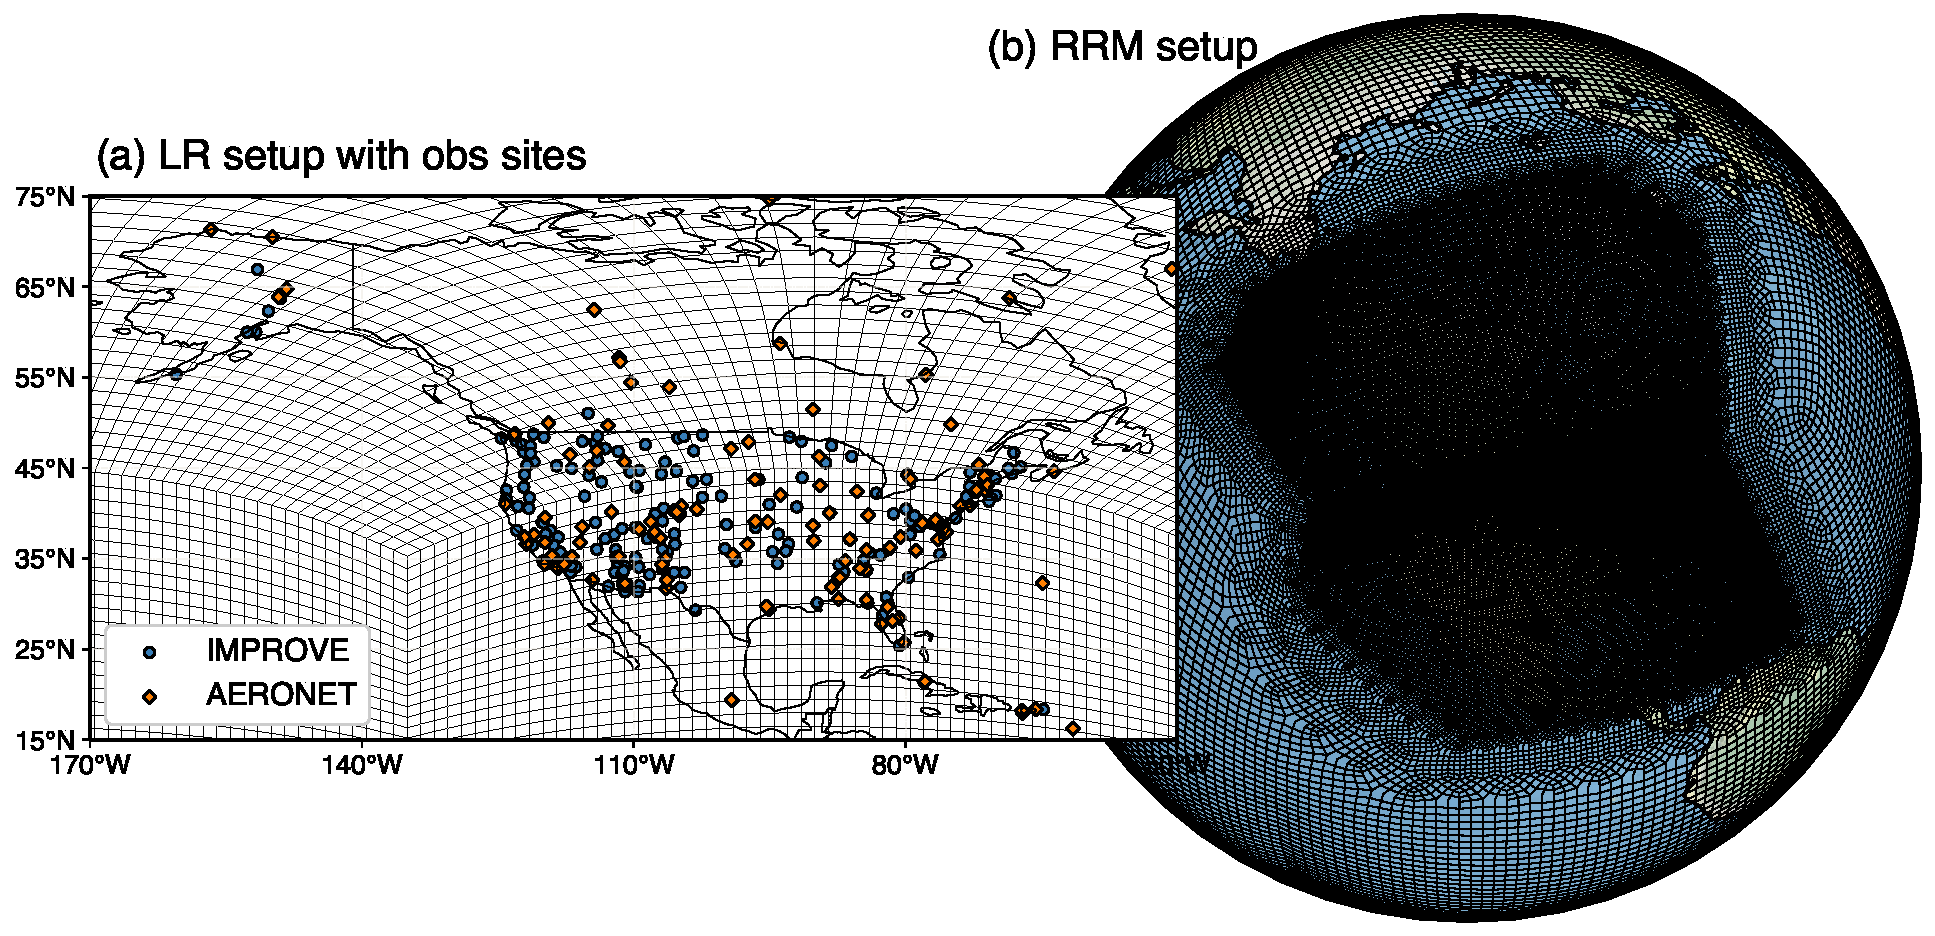
\includegraphics[width=18cm]{fig01.png}
\caption{The model-native grid configuration for (a) low-resolution, LR (ne30pg2) grid, and (b) regionally refined mesh over North America (NA RRM) are shown. The locations for point-source aerosol measurement sites over North America from IMPROVE and AERONET data set are also shown overlaid on the LR grid in panel (a).}
\end{figure}

\clearpage
\begin{figure}[t]
%\includegraphics[width=17cm]{fig02.pdf}
\caption{Flowcharts illustrating how the aerosols and precursor gas emission is handled in the EAMv2 simulation. Light green boxes in panel (a) depicts the modules impacted during one time step of the physics and dynamics calculations. Panel (b) compares the default and the new emission treatment. The key differences are depicted by light orange and light blue boxes for default and new emission treatment respectively.}
\end{figure}

\clearpage
\begin{figure}[t]
%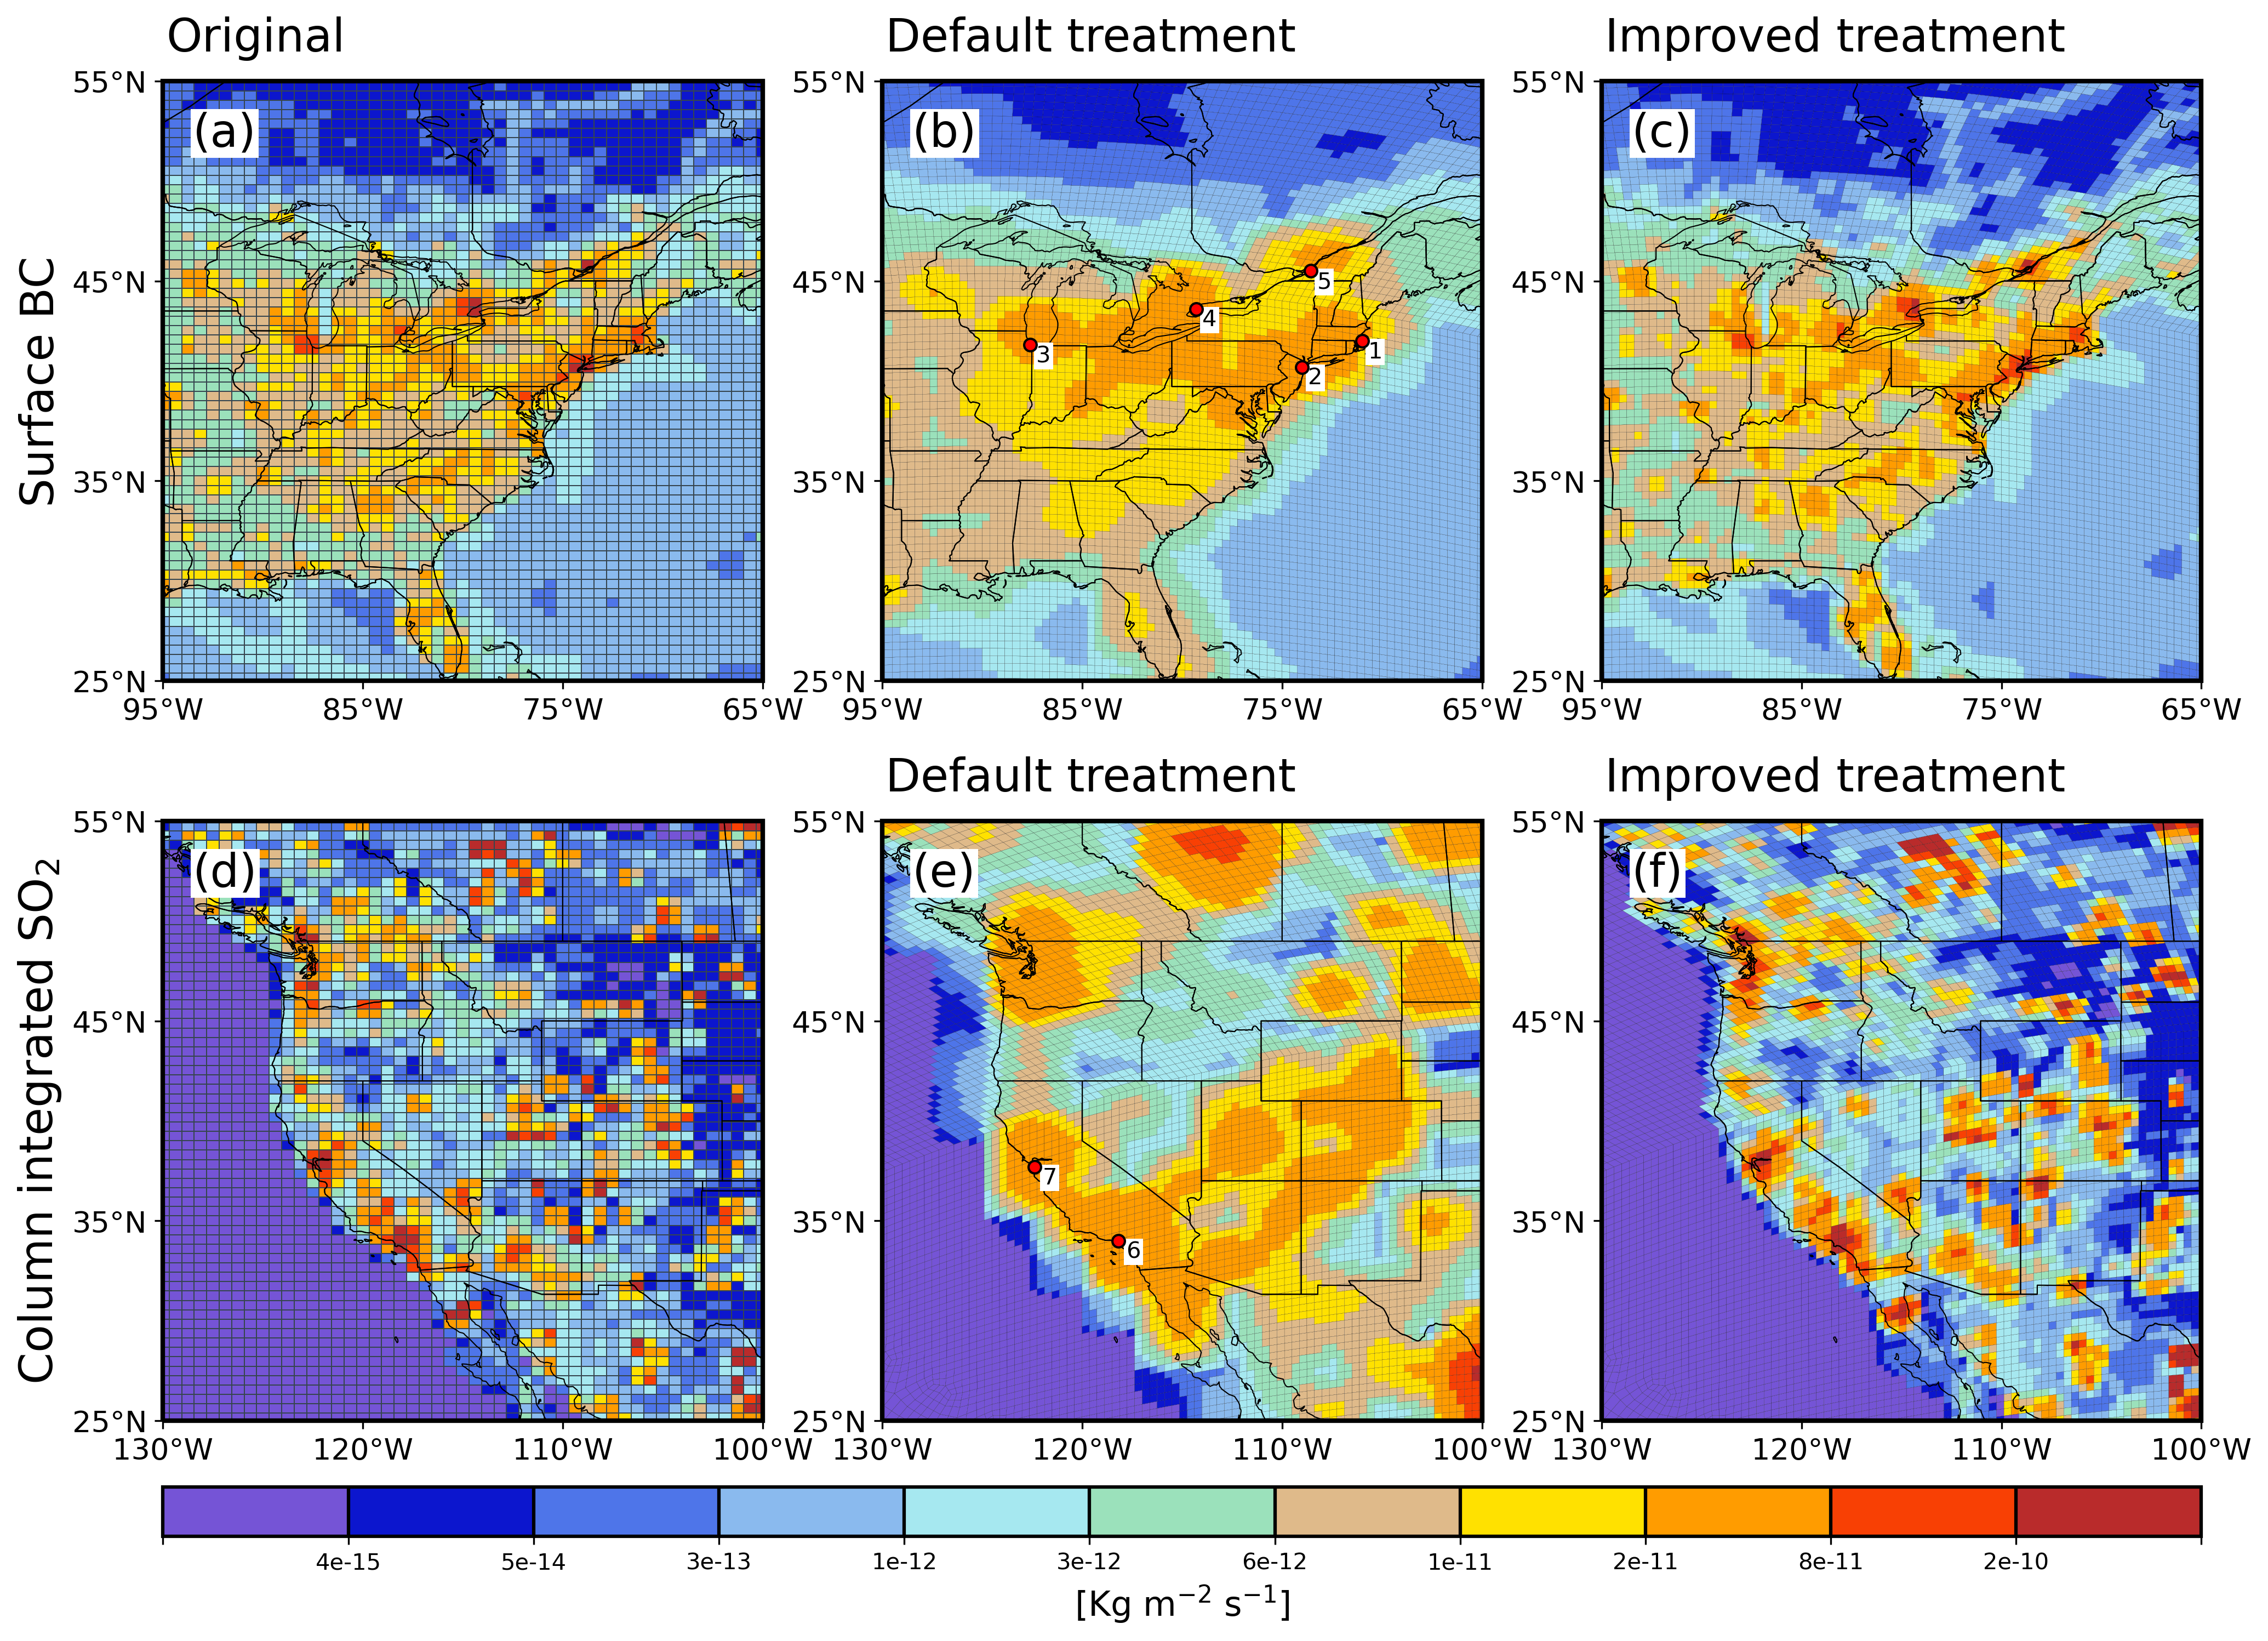
\includegraphics[width=17.5cm]{fig03.png}
\caption{Spatial distribution of the present-day surface BC emissions (top) and column integrated SO2 emissions (bottom) from the original high-resolution data (a, d), the default emission treatment (b, e), and the improved emission treatment (c, f) for RRM simulations. Distributions are shown over eastern (western) United States for BC (SO2) emissions in Kg/m2/s units. Red circles in panel b and e indicate major cities with large surface BC and SO2 emissions respectively. Markers titled 1, 2, 3, 4, 5, 6 and 7 depict Boston, New York, Chicago, Toronto, Montreal, Los Angeles, and San Francisco respectively.}
\end{figure}

\clearpage
\begin{figure}[t]
%\includegraphics[width=17.5cm]{fig04.png}
\caption{Simulated spatial distribution of annual mean aerosol surface concentration from RRM-PD (left column) and the relative difference between RRM-SE-PD and RRM-PD (right column) over North America. Distributions are shown for (a, b) Black Carbon (BC), (c, d) Primary Organic Matter (POM), and (e, f) Sulfate aerosols. The relative difference for field X is calculated as: $(\frac{X_{se}-X_{def}}{X_{def}}) \times 100 \%$, where “se” and “def” subscripts refer to the simulations with new and default emission treatment respectively. Mean, RMSE and normalized RMSE (N\_RMSE) are indicated at the top right corner of the panels. Mean and RMSE has a unit of $\mu{g}\ m^{-3}$. N\_RMSE is defined as in Table 2.}
\end{figure}

\clearpage
\begin{figure}[t]
%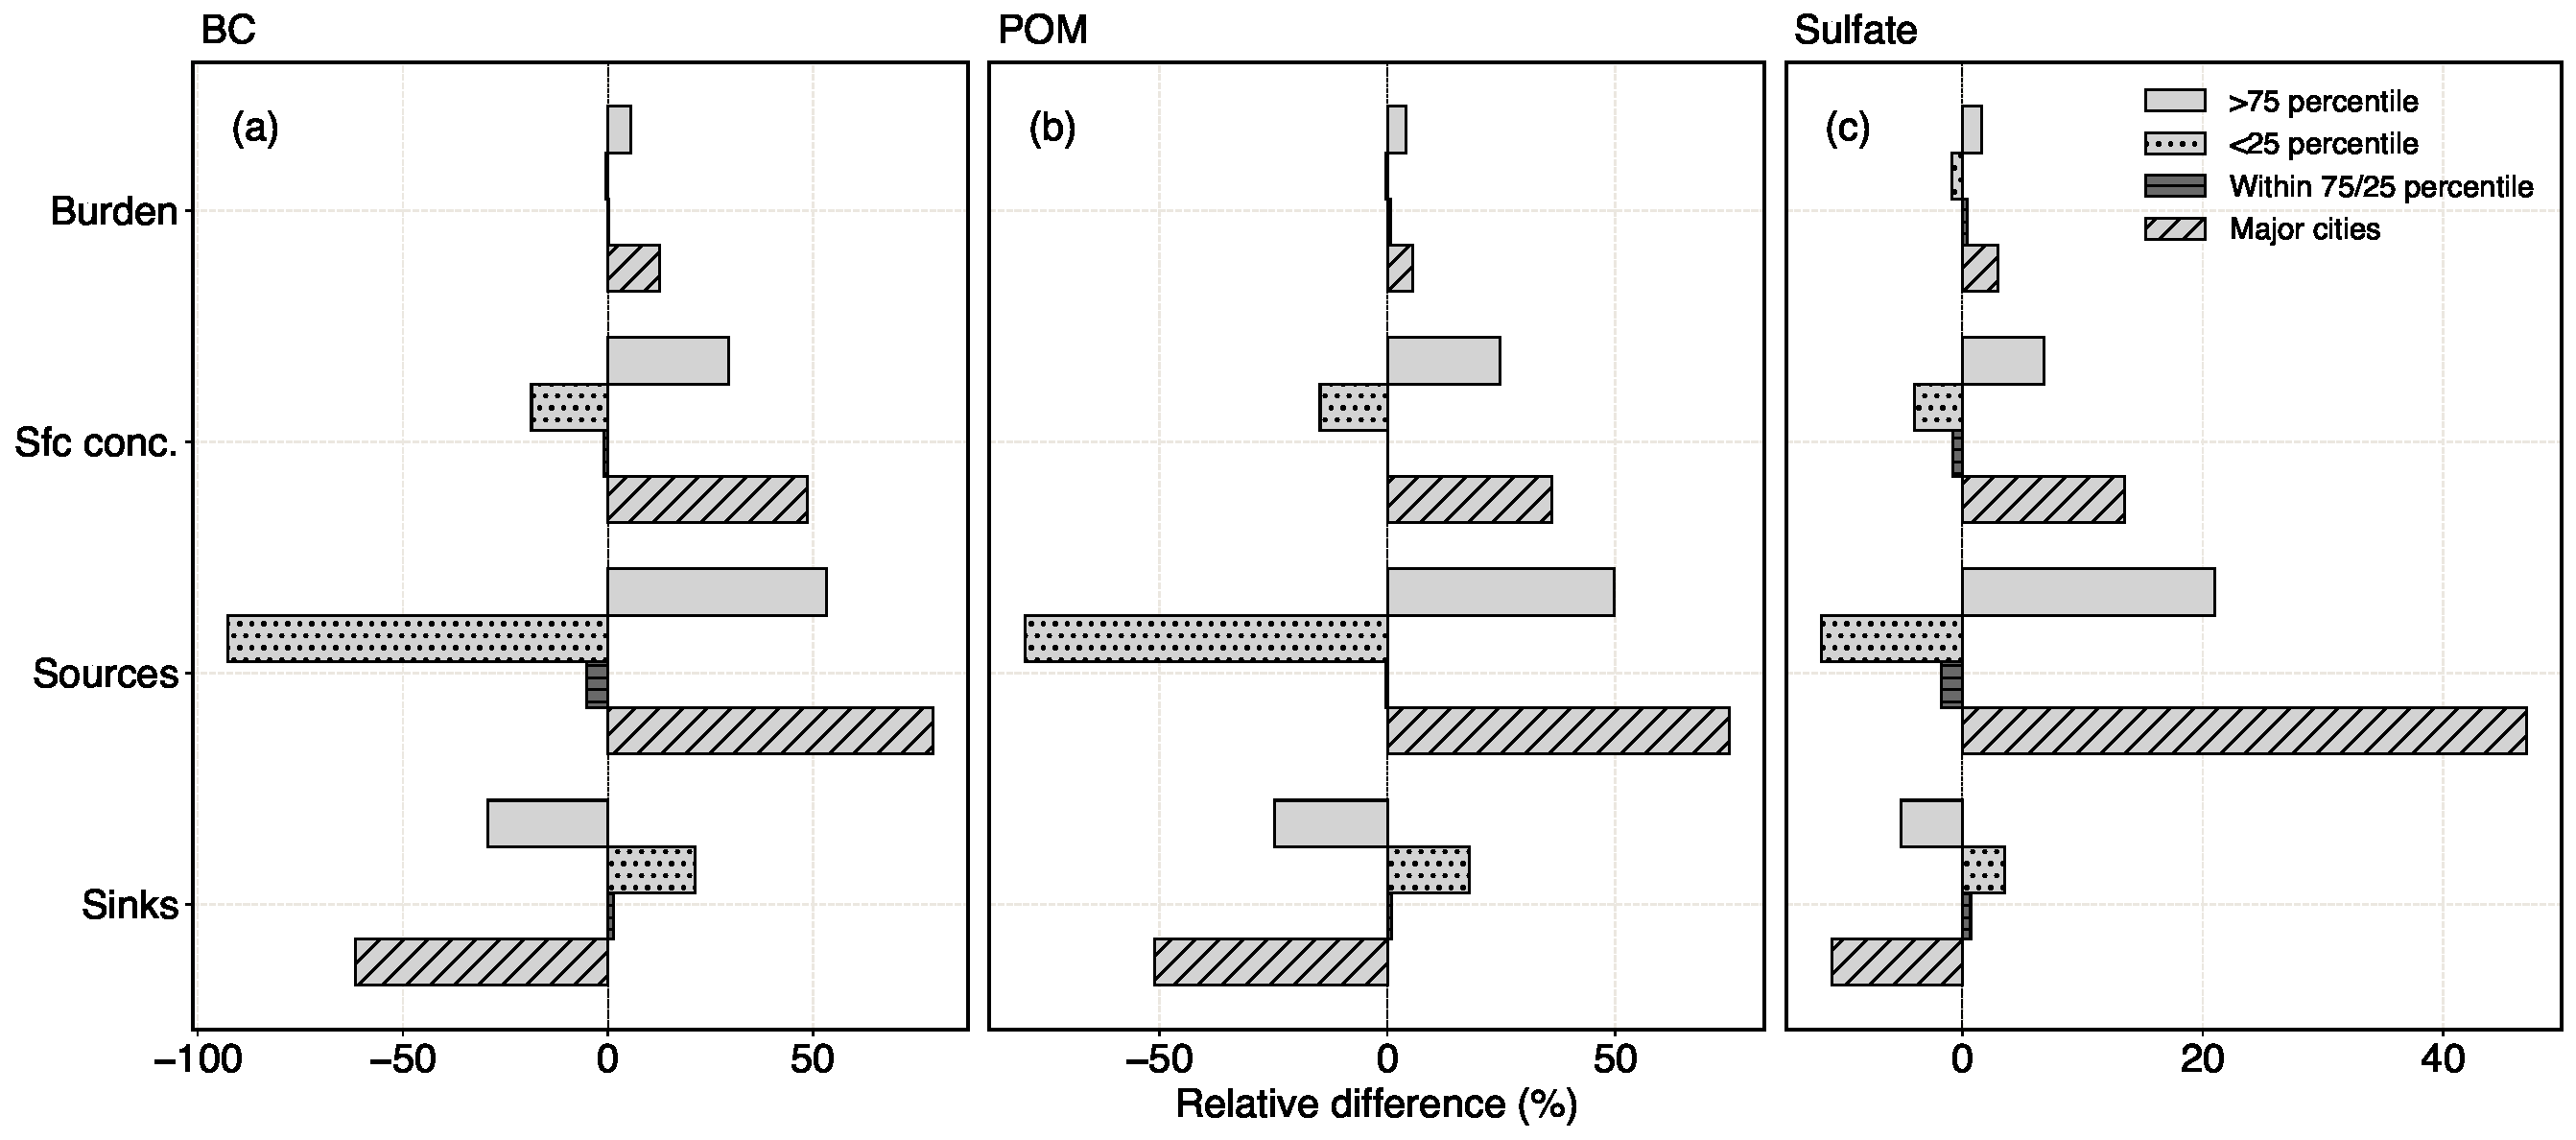
\includegraphics[width=17.5cm]{fig05.pdf}
\caption{Quantitative distribution of annual mean relative differences between RRM-SE-PD and RRM-PD for simulated aerosol burden, surface concentration, aerosol sources and aerosol sinks. Distributions are shown for (a) BC, (b) POM, and (c) sulfate aerosols in percentage. Simulated fields are masked by emission differences between the new and default treatment. Masking is applied for regions above 75th percentile (>75 percentile), below 25th percentile (<25 percentile), and within 25/75th percentiles over North America. Urban-scale differences are also shown considering major cities with larger anthropogenic aerosol emissions.}
\end{figure}

\clearpage
\begin{figure}[t]
%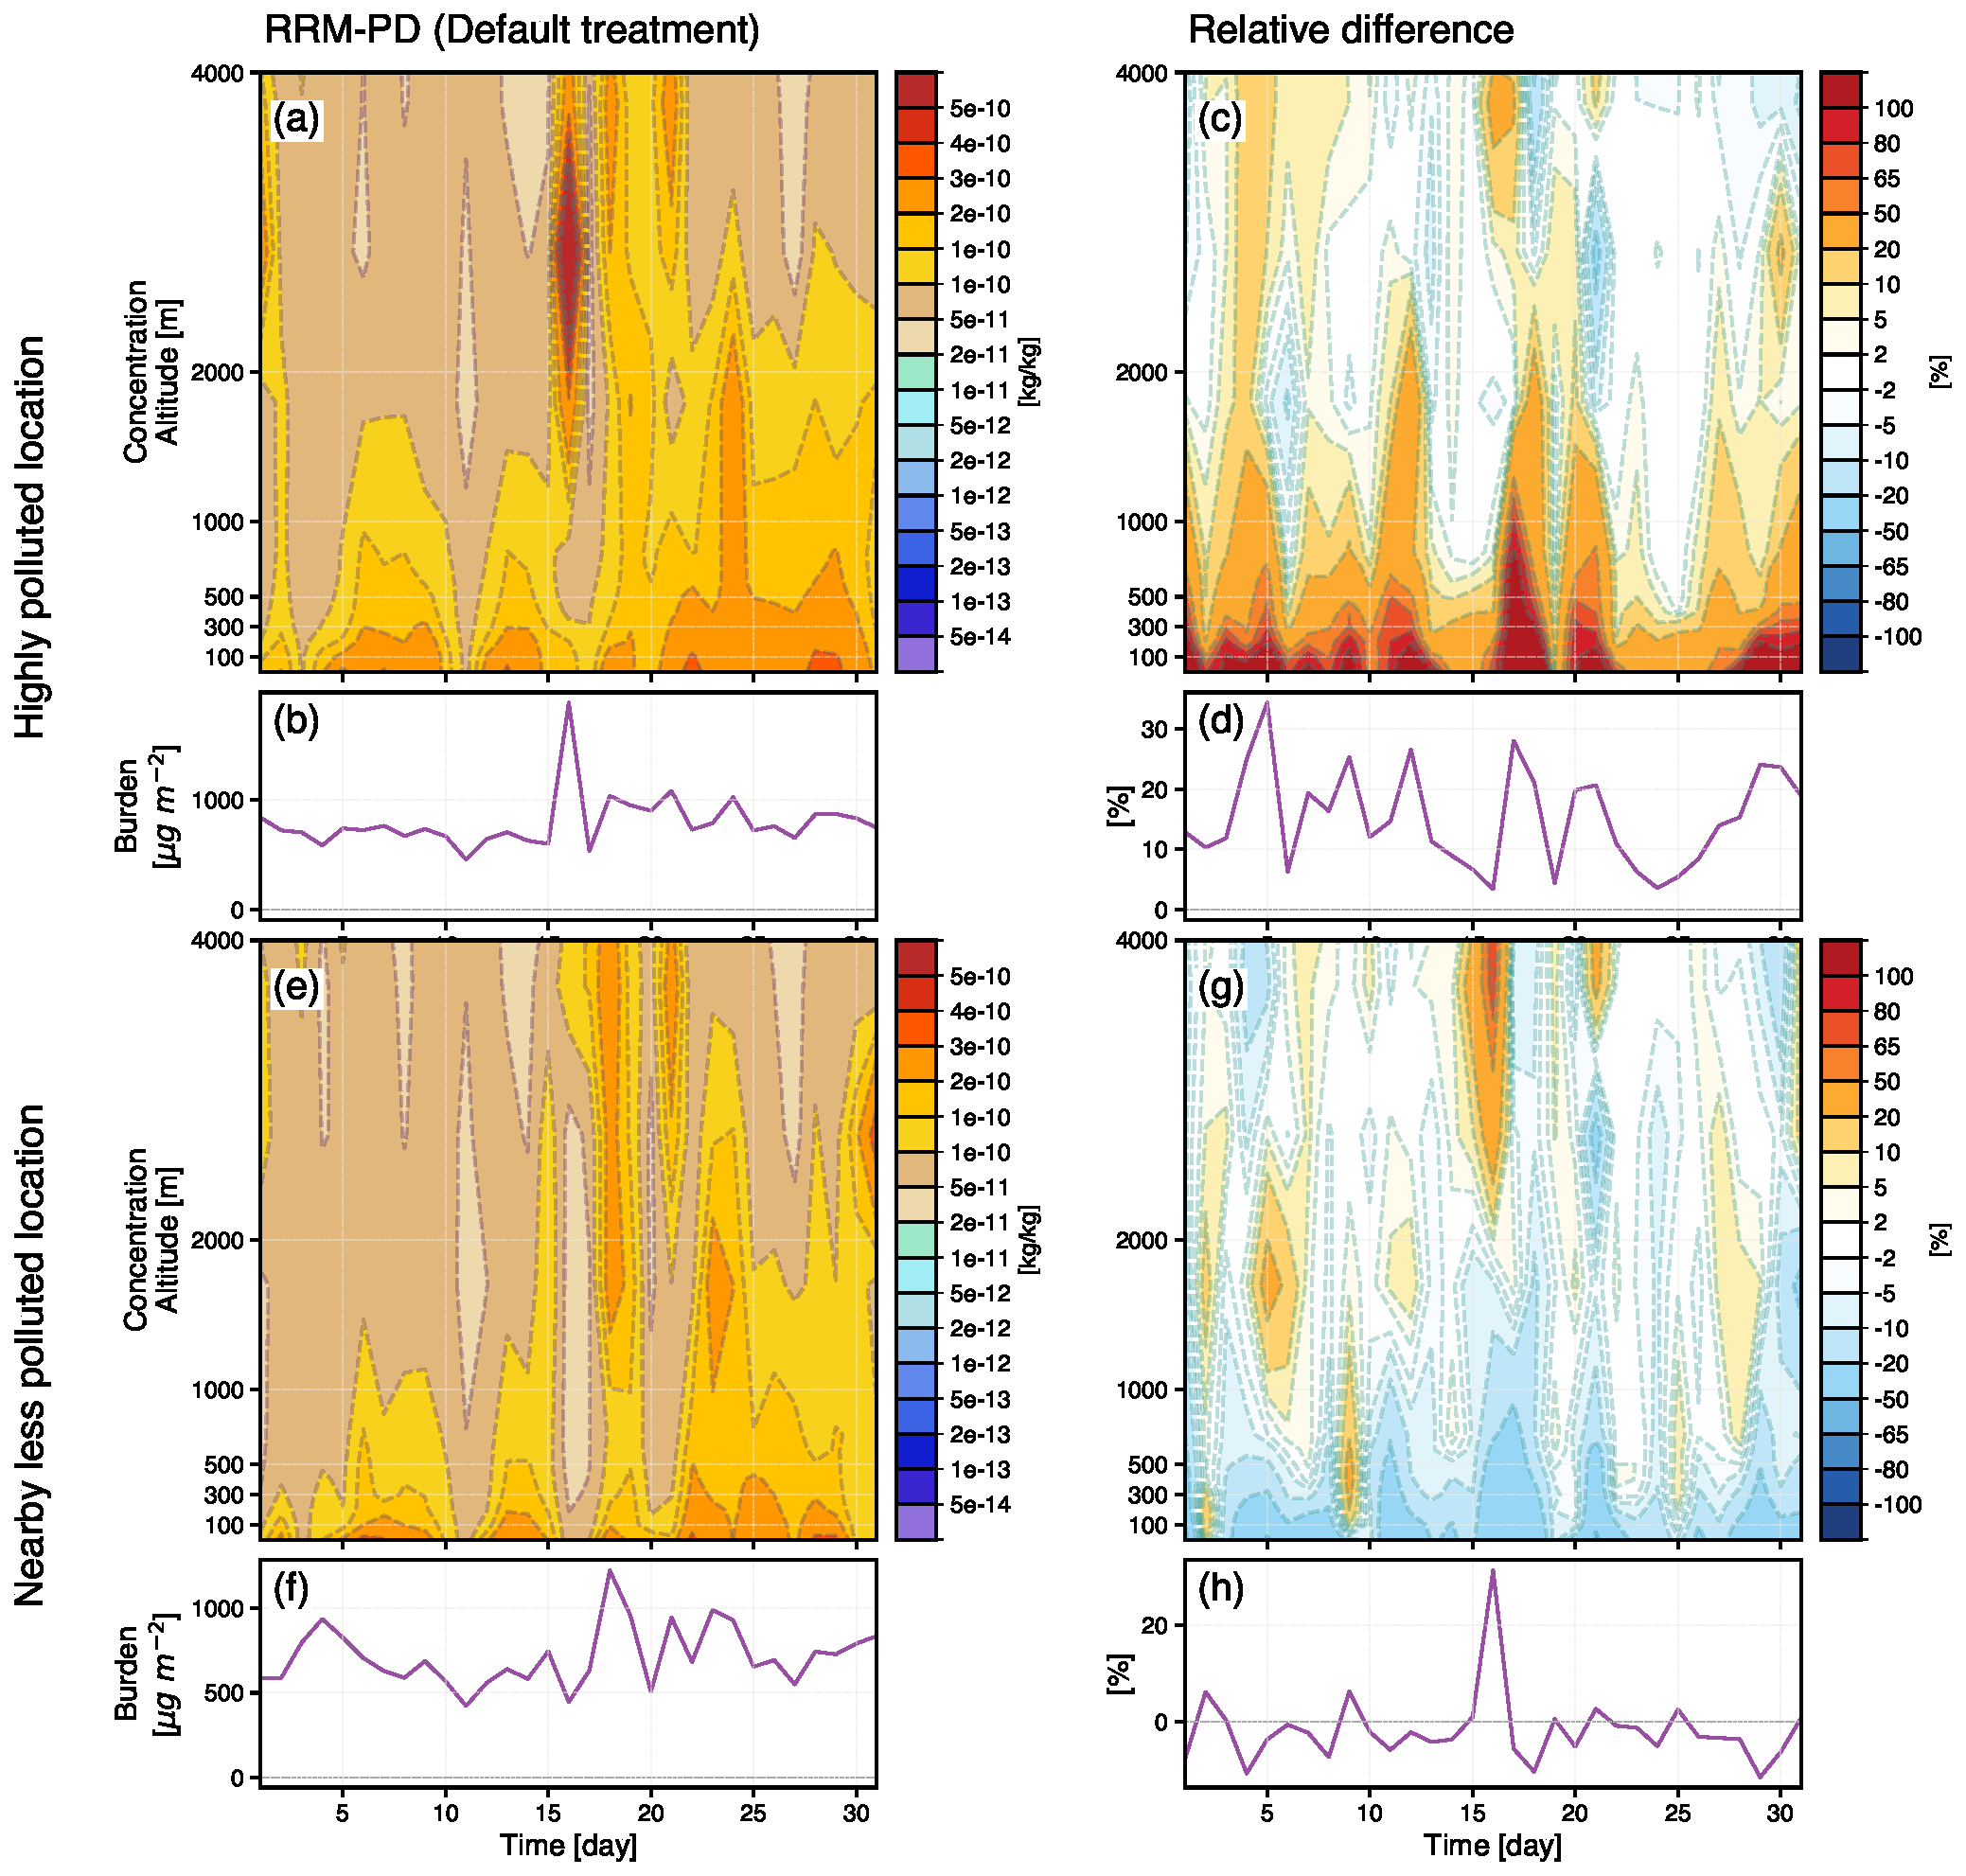
\includegraphics[width=17.5cm]{fig06.pdf}
\caption{Daily mean Black carbon (BC) concentration profile and burden time-series during the month of July of 2016 near sharp spatial emission gradient in eastern North America. Simulated vertical distribution and burden time-series from RRM-PD (left column) and the relative difference between RRM-SE-PD and RRM-PD (right column) are shown. Panels a-d depicts highly polluted location, with panels e-h depicting nearby less polluted location.}
\end{figure}

\clearpage
\begin{figure}[t]
%\includegraphics[width=15cm]{fig07.png}
\caption{Spatial distribution of annual mean simulated (a, b) aerosol extinction at surface, (c, d) aerosol absorption at surface, (e, f) Aerosol Optical Depth (AOD), and (g, h) absorbing AOD from RRM-PD (left column) and the relative difference between RRM-SE-PD and RRM-PD (right column) over North America. The relative difference for field X is calculated as: $(\frac{X_{se}-X_{def}}{X_{def}}) \times 100 \%$, where “se” and “def” subscripts refer to the simulations with new and default emission treatment respectively. Mean, RMSE and normalized RMSE (N\_RMSE) are indicated at the top right corner of the panels. Mean and RMSE has a unit of $\mu{g}\ m^{-3}$. N\_RMSE is defined as in Table 2.}
\end{figure}

\clearpage
\begin{figure}[t]
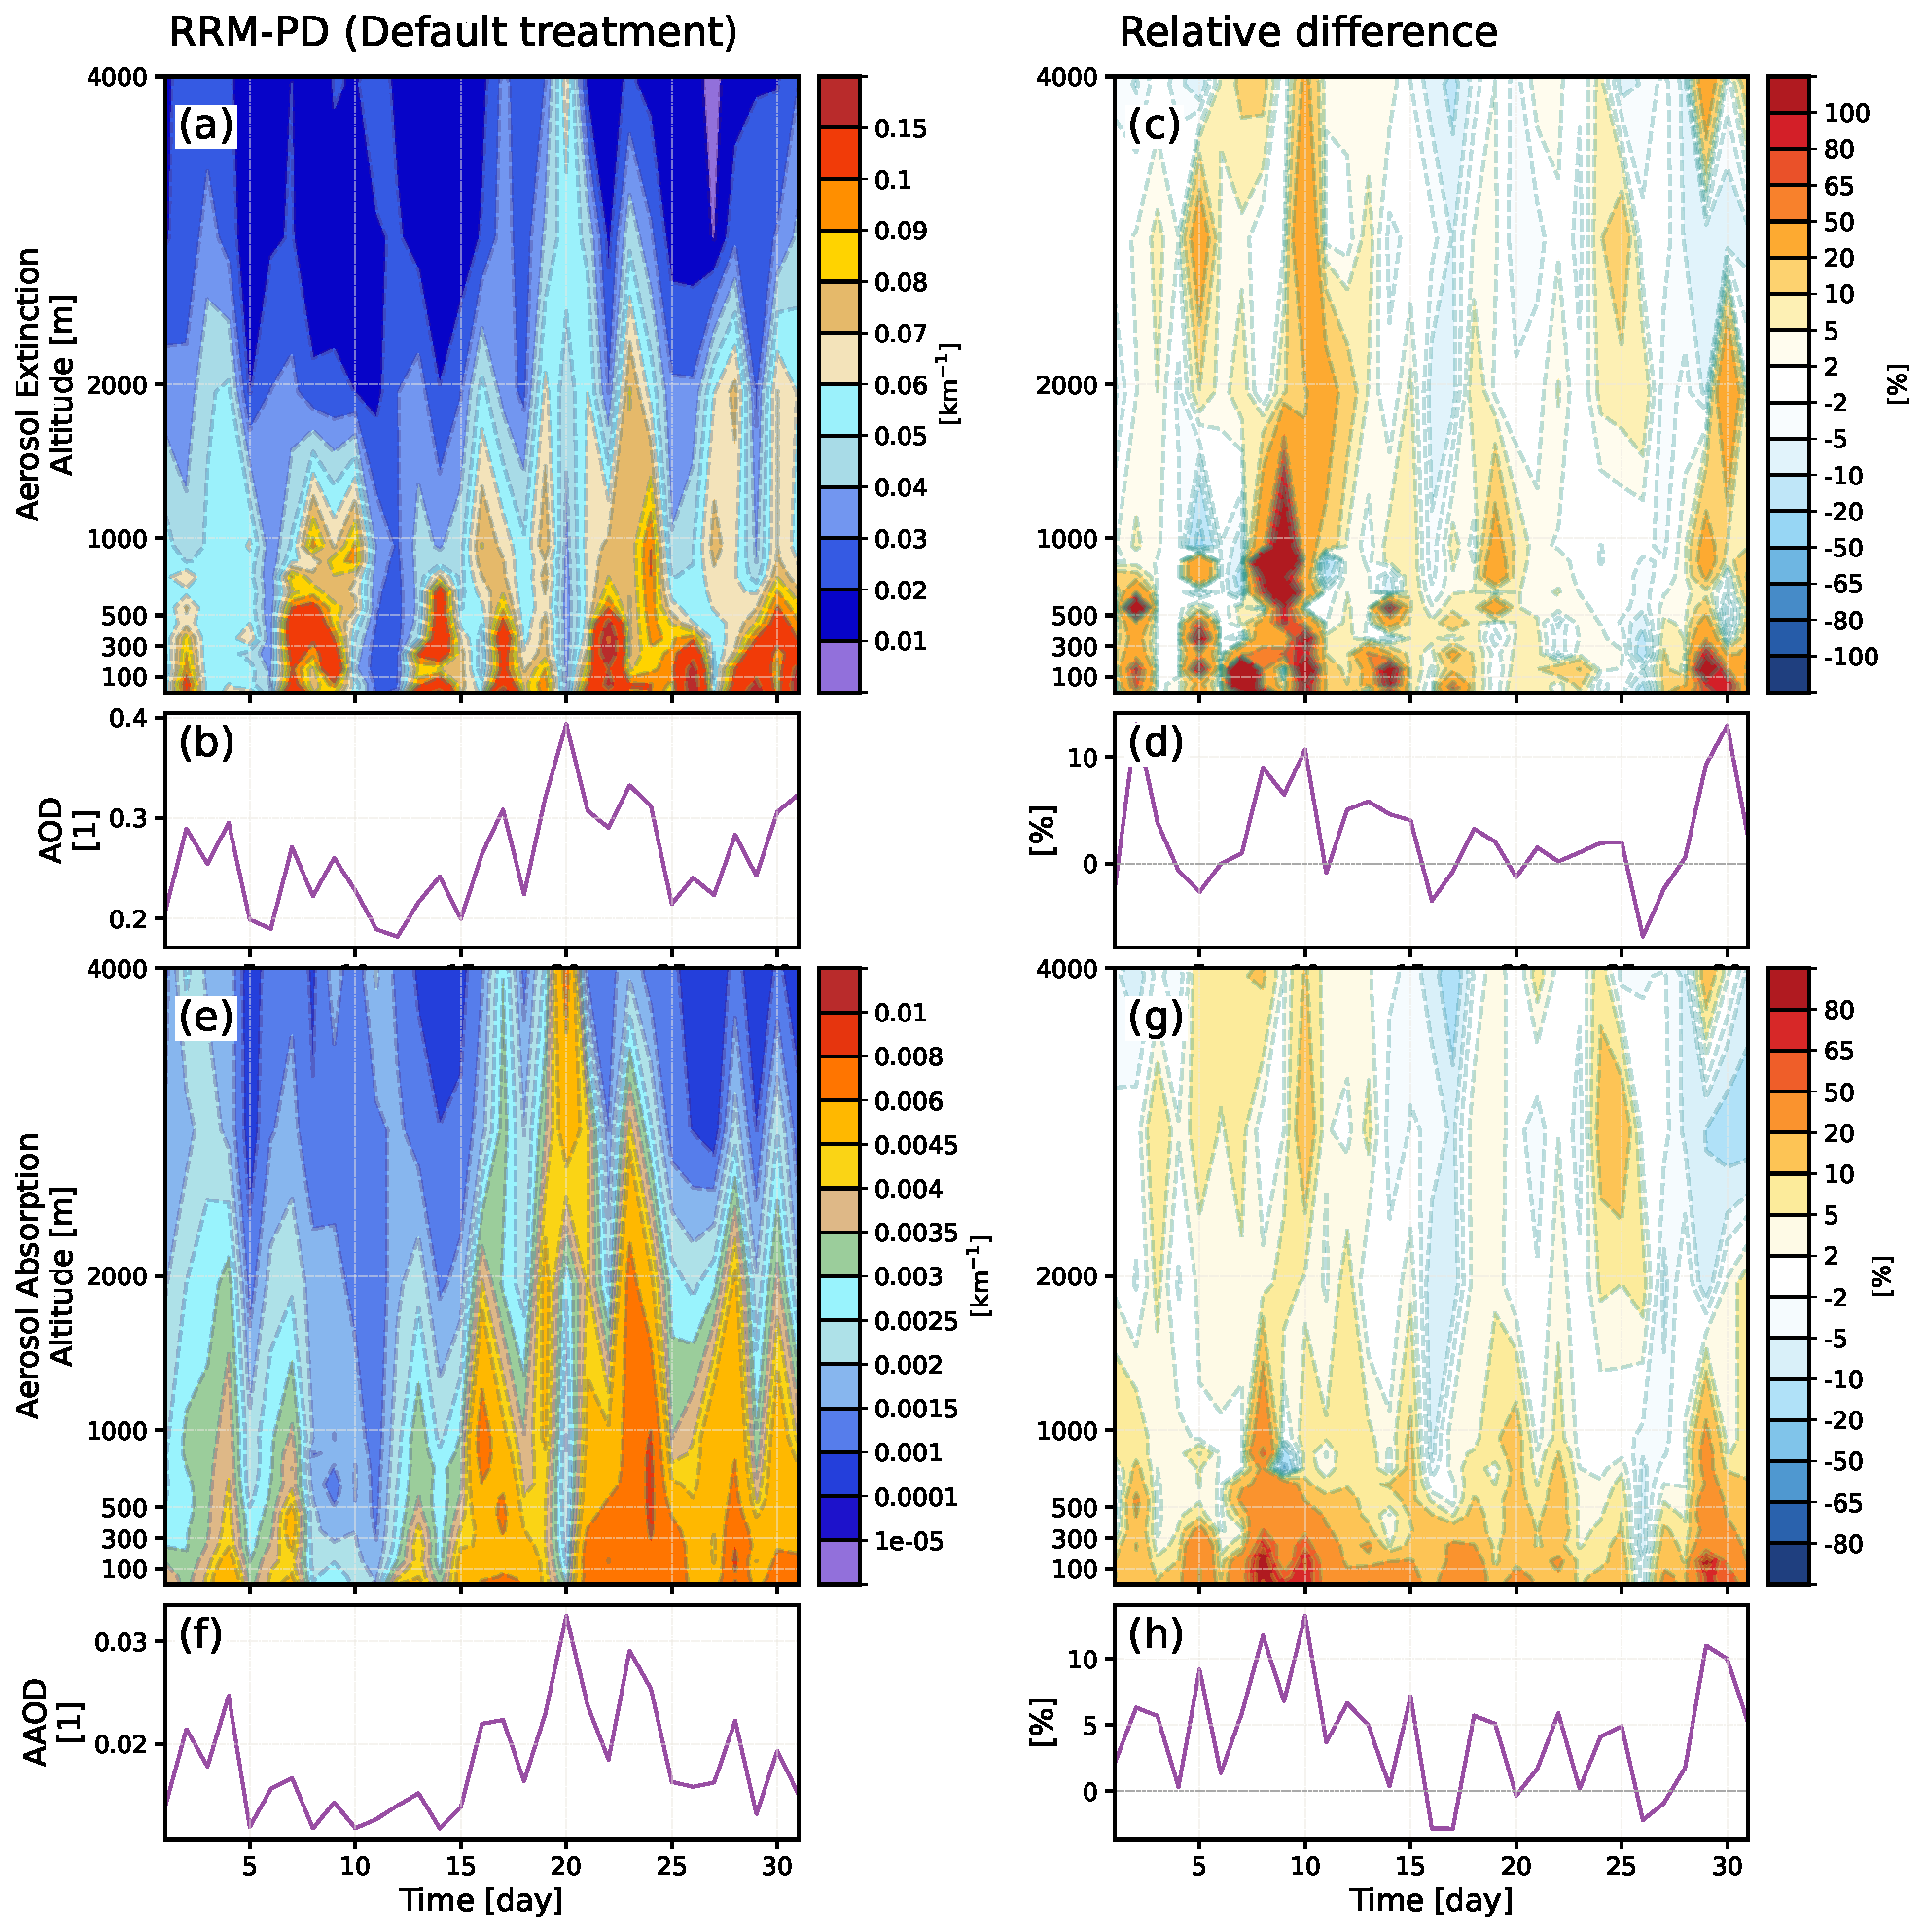
\includegraphics[width=17.5cm]{fig08.pdf}
\caption{Daily mean aerosol extinction and absorption time-series during the month of July of 2016 near sharp spatial emission gradient in northeast United States. Simulated aerosol extinction profile, absorption profile, AOD, and absorption AOD (AAOD) time-series from RRM-PD (left column) and the relative difference between RRM-SE-PD and RRM-PD (right column) are shown.}
\end{figure}

\clearpage
\begin{figure}[t]
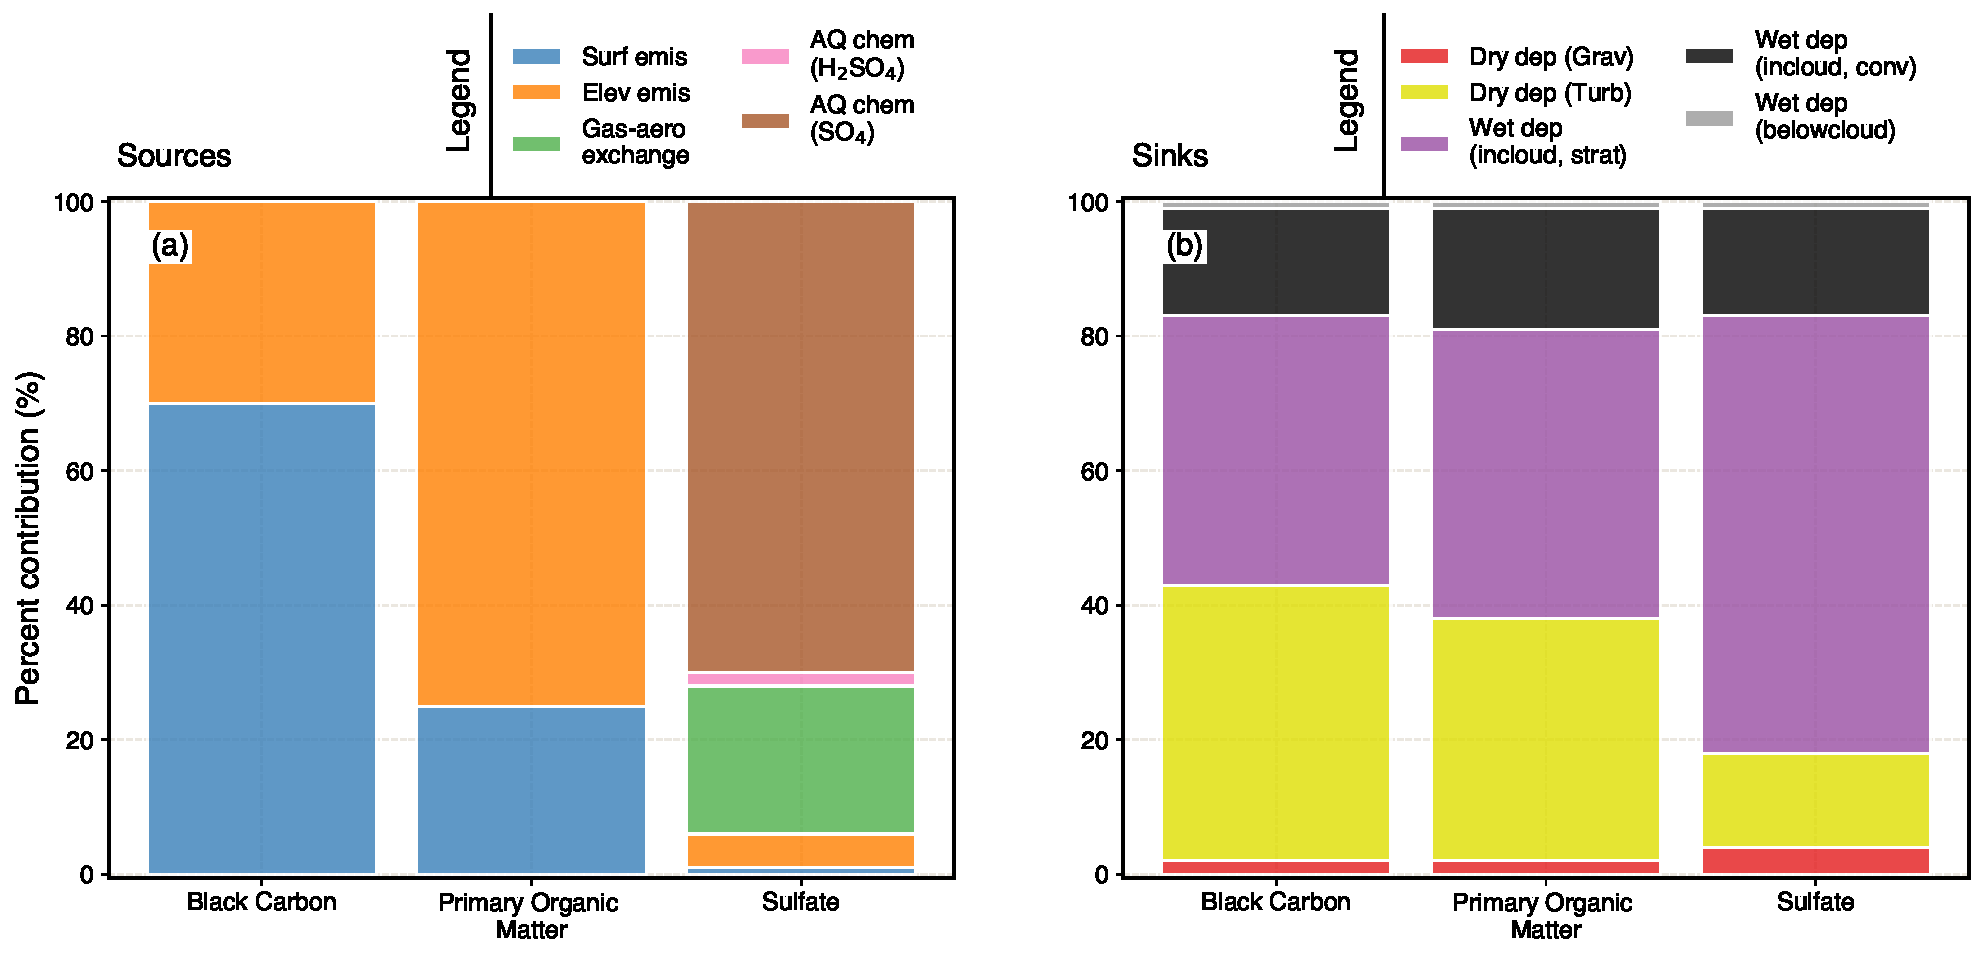
\includegraphics[width=17.5cm]{fig09.pdf}
\caption{Contribution of the decomposed aerosol source and sink processes in EAMv2 simulations for Black Carbon (BC), Primary Organic Matter (POM), and Sulfate (SO4) aerosols. All estimates are from annual means over North America. Legend for sources and sinks are shown separately at the top right corner of each panel. Decomposed dry deposition processes “Grav” and “Turb” refers to the gravitational settling and turbulent deposition respectively.}
\end{figure}

\clearpage
\begin{figure}[t]
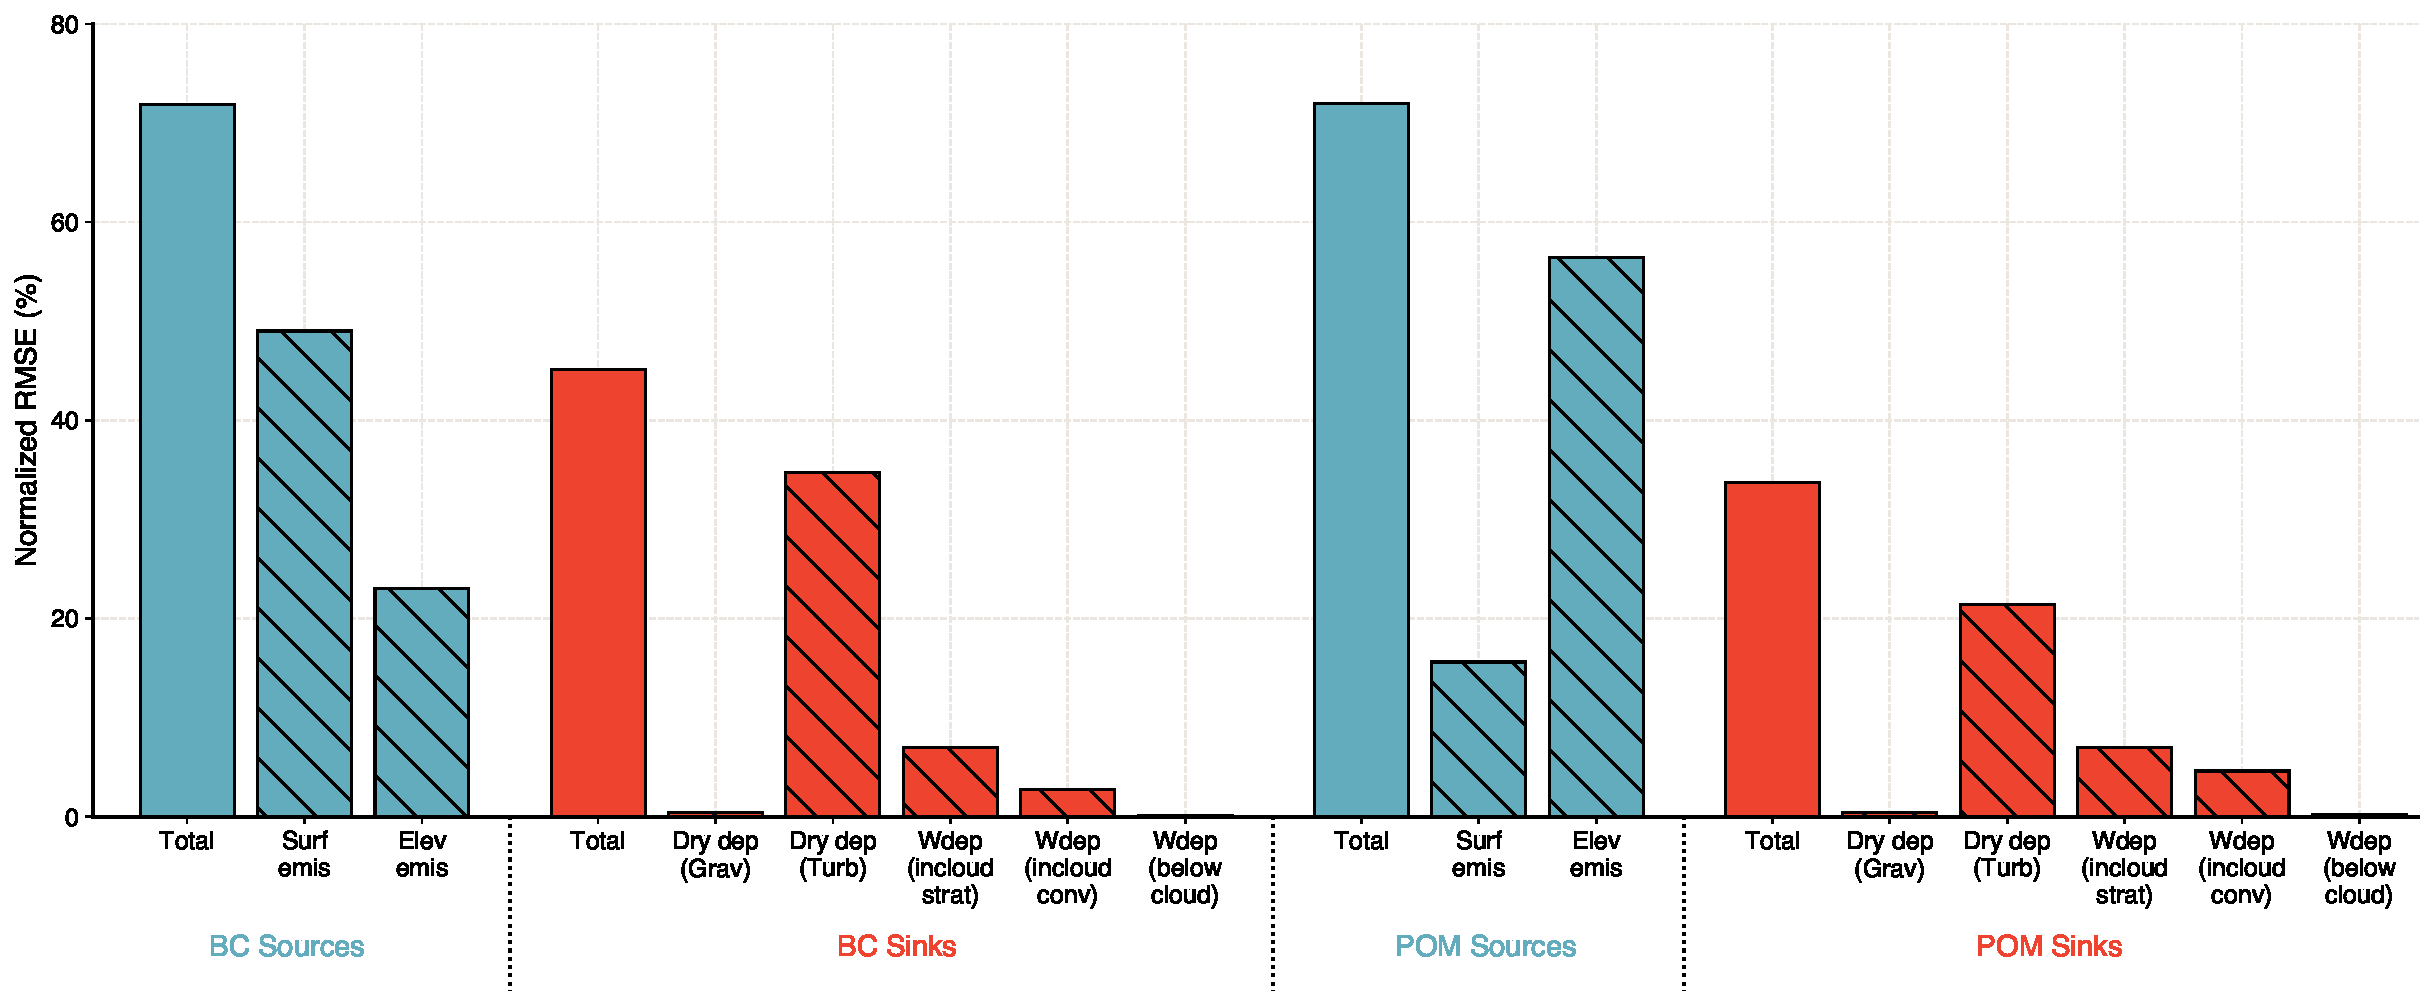
\includegraphics[width=17.5cm]{fig10.pdf}
\caption{Error estimates of the total and decomposed processes contributing to the simulated sources and sinks of BC and POM from present-day (PD) RRM simulations. All RMSE estimates are over the North America land surface. Normalized RMSE is defined as $N\_RMSE_{Total} \times \frac{Weight_{i} \times N\_RMSE_{i}}{\sum{(Weight_{i} \times N\_RMSE_{i})}}$ , where N\_RMSE is defined as in Table 2, weights are from Figure 6, and subscript “i” indicates decomposed process. The solid bars represent the normalized RMSE for the total source and sink. The hatched bars are the decomposed processes normalized to the total N\_RMSE values. The “Wdep” bars refer to the wet deposition components.}
\end{figure}

\clearpage
\begin{figure}[t]
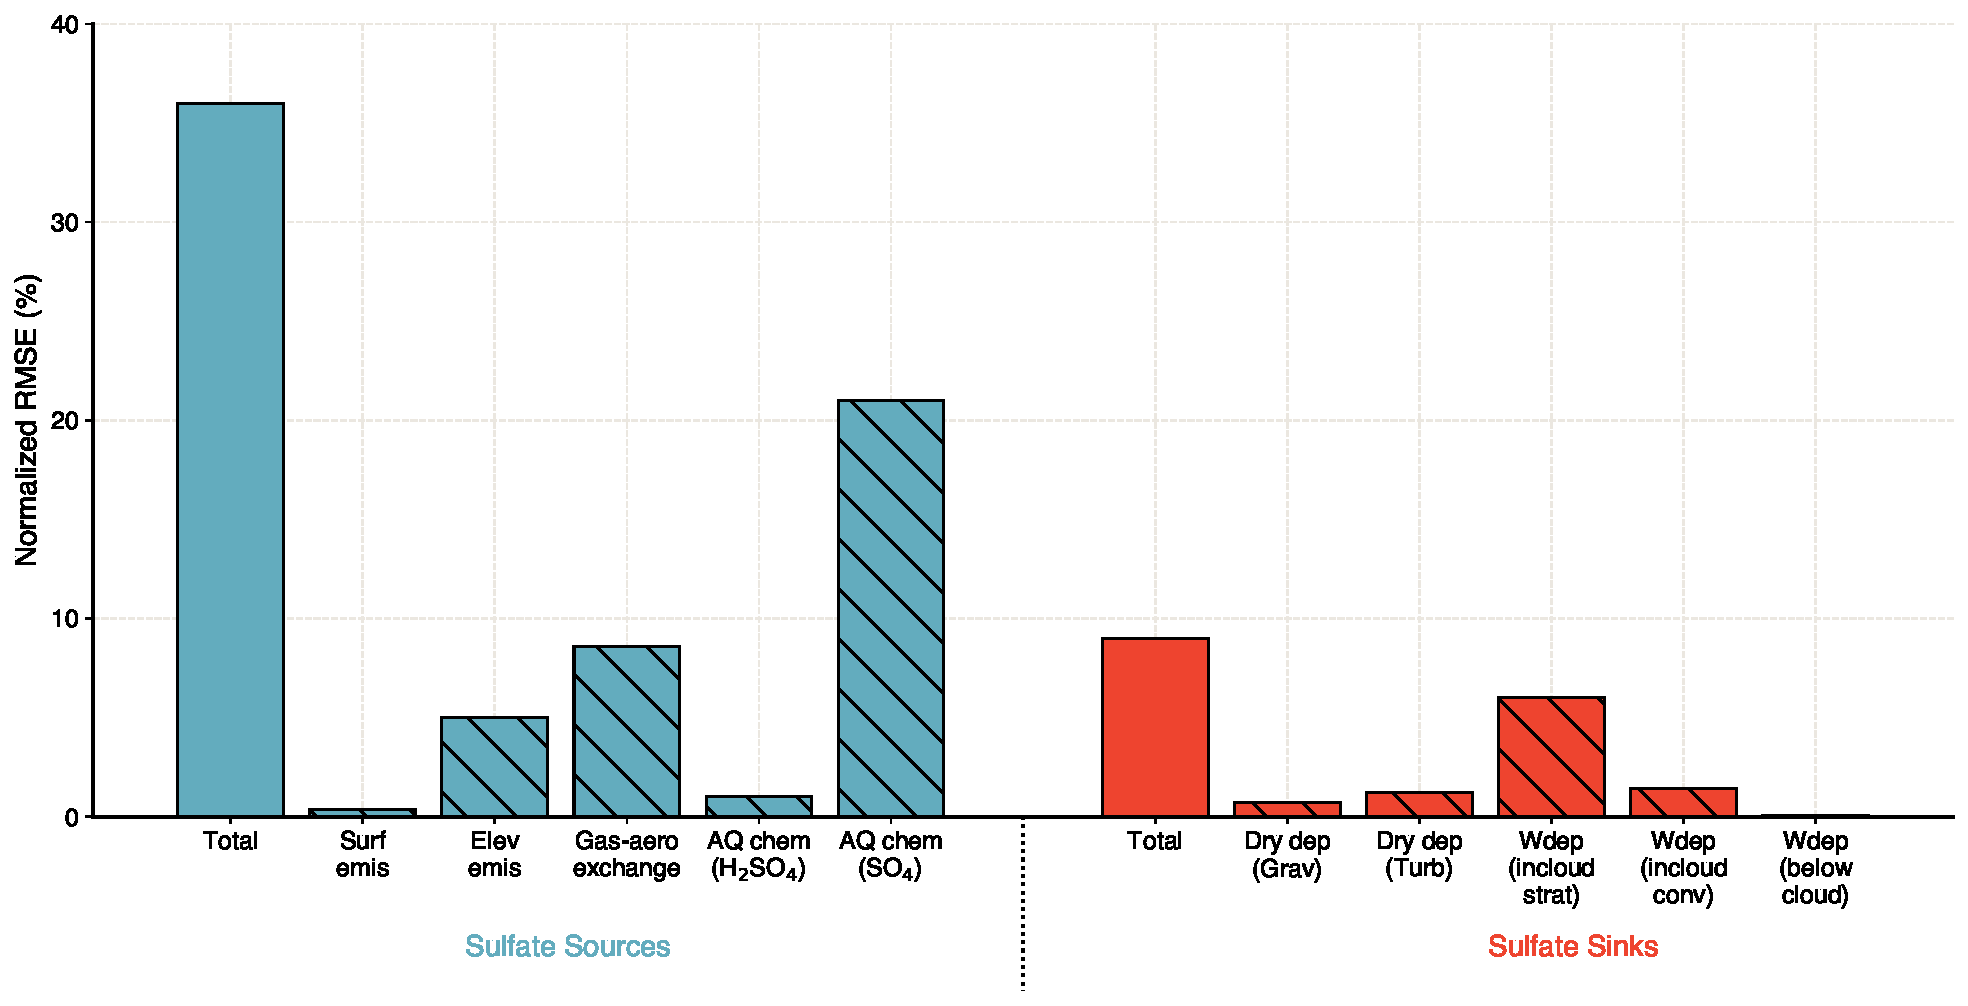
\includegraphics[width=17.5cm]{fig11.pdf}
\caption{Error estimates of the total and decomposed processes contributing to the simulated sources and sinks of Sulfate aerosols from present-day (PD) RRM simulations. All RMSE estimates are over the North America land surface. Normalized RMSE is defined as $N\_RMSE_{Total} \times \frac{Weight_{i} \times N\_RMSE_{i}}{\sum{(Weight_{i} \times N\_RMSE_{i})}}$ , where N\_RMSE is defined as in Table 2, weights are from Figure 6, and subscript “i” indicates decomposed process. The solid bars represent the normalized RMSE for the total source and sink. The hatched bars are the decomposed processes normalized to the total N\_RMSE values. The “Wdep” bars refer to the wet deposition components.}
\end{figure}

\clearpage
\begin{figure}[t]
\includegraphics[width=16.5cm]{fig12.pdf}
\caption{Scatter plots between simulated and observed monthly mean surface concentrations of (a, c) Black Carbon (BC) and (b, d) Primary Organic Matter (POM). Observations of the surface concentrations are from IMPROVE for the simulation year of 2016. Scatter plot statistics compare the spearman’s correlation (R), number of data points (n), RMSE, NMB values between (a, b) RRM-PD and (c, d) RRM-SE-PD simulation. RMSE and NMB are defined as in Table 2. Solid lines indicate the 1:1 ratio, and the dashed lines indicate the 1:2 and 2:1 ratio. The values at the top of each column indicate the observed mean.fig14}
\end{figure}

\clearpage
\begin{figure}[t]
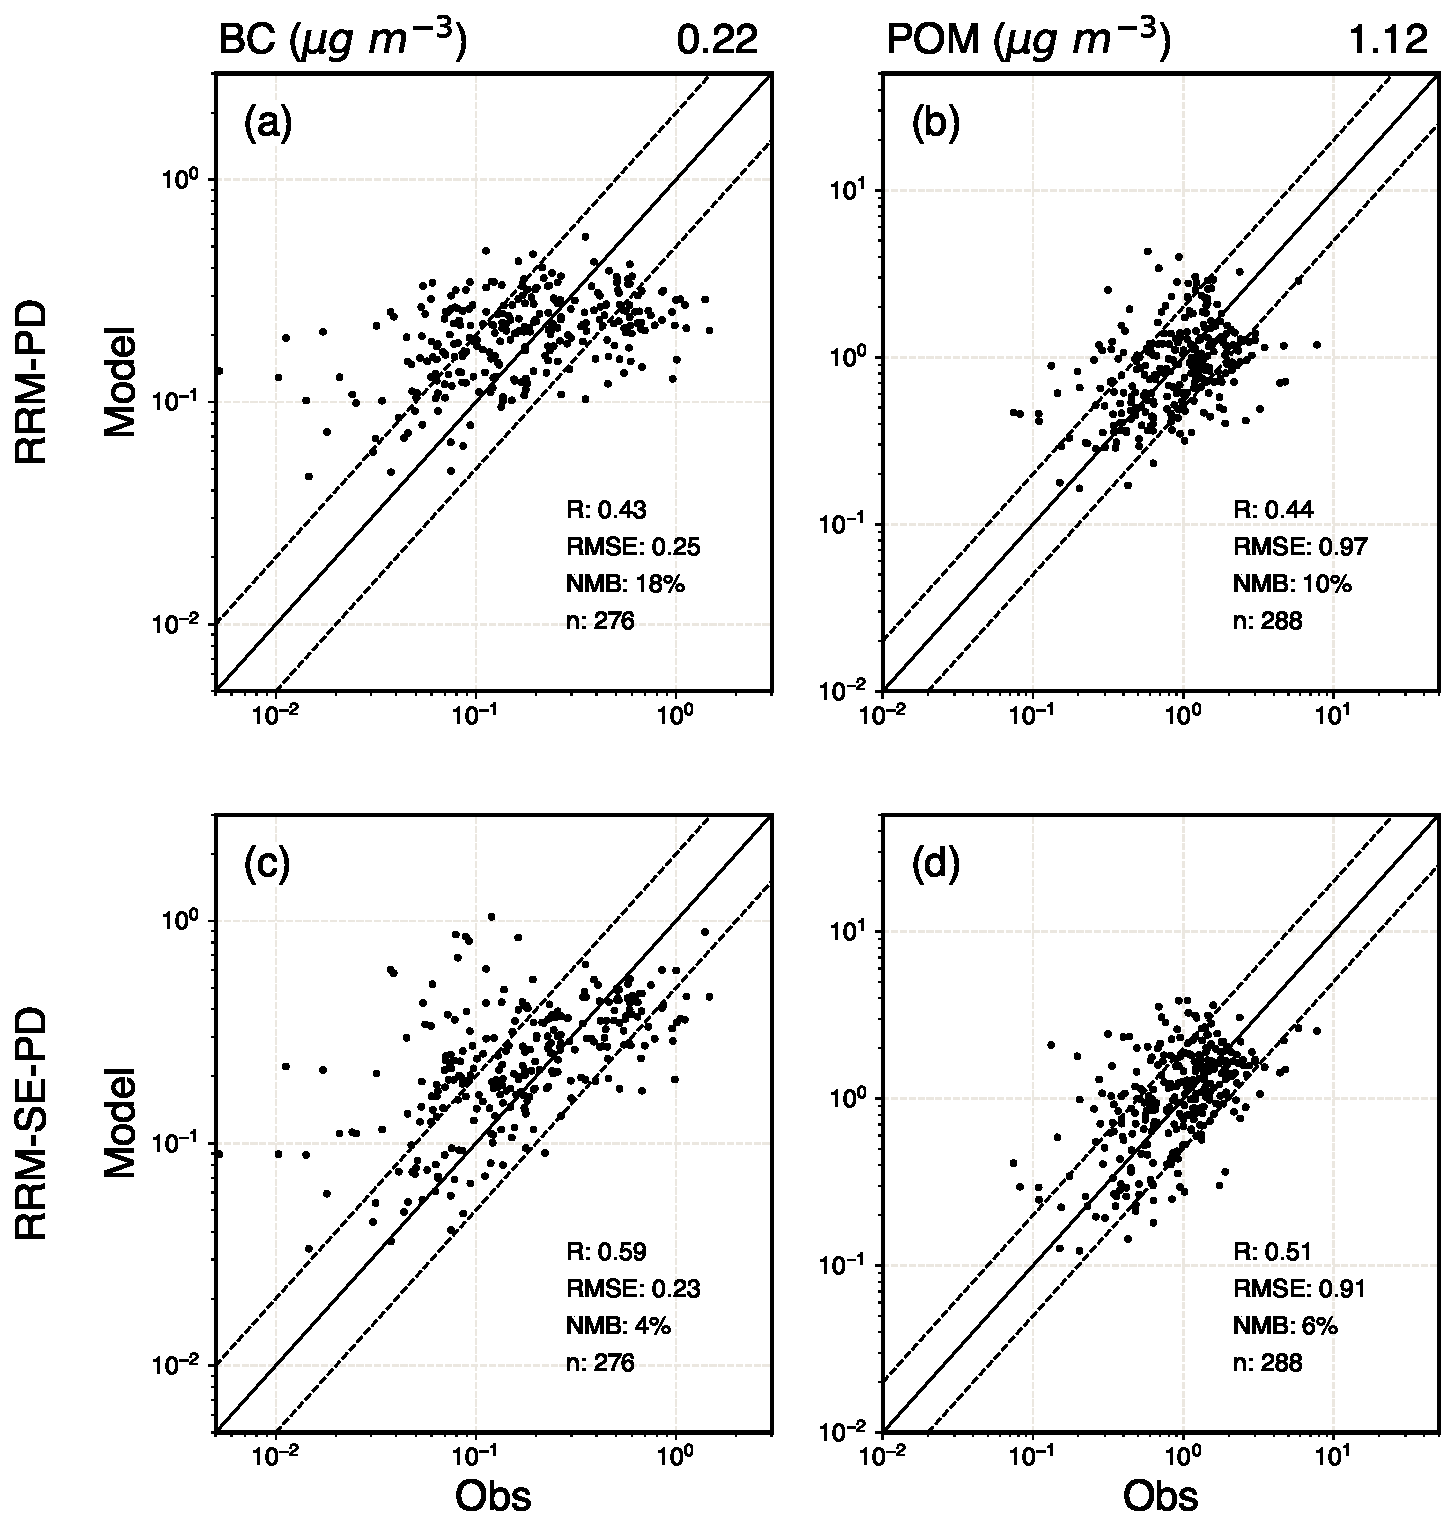
\includegraphics[width=17cm]{fig13.pdf}
\caption{Boxplot comparison of the daily mean distribution for (a) BC and (b) POM surface concentrations from RRM-PD simulation, RRM-SE-PD simulation and IMPROVE network measurements. The whiskers are based on 1.5 times interquartile range (IQR). Distributions are plotted for different seasons over the simulation year, with red diamonds indicating the seasonal means.}
\end{figure}

\clearpage
\begin{figure}[t]
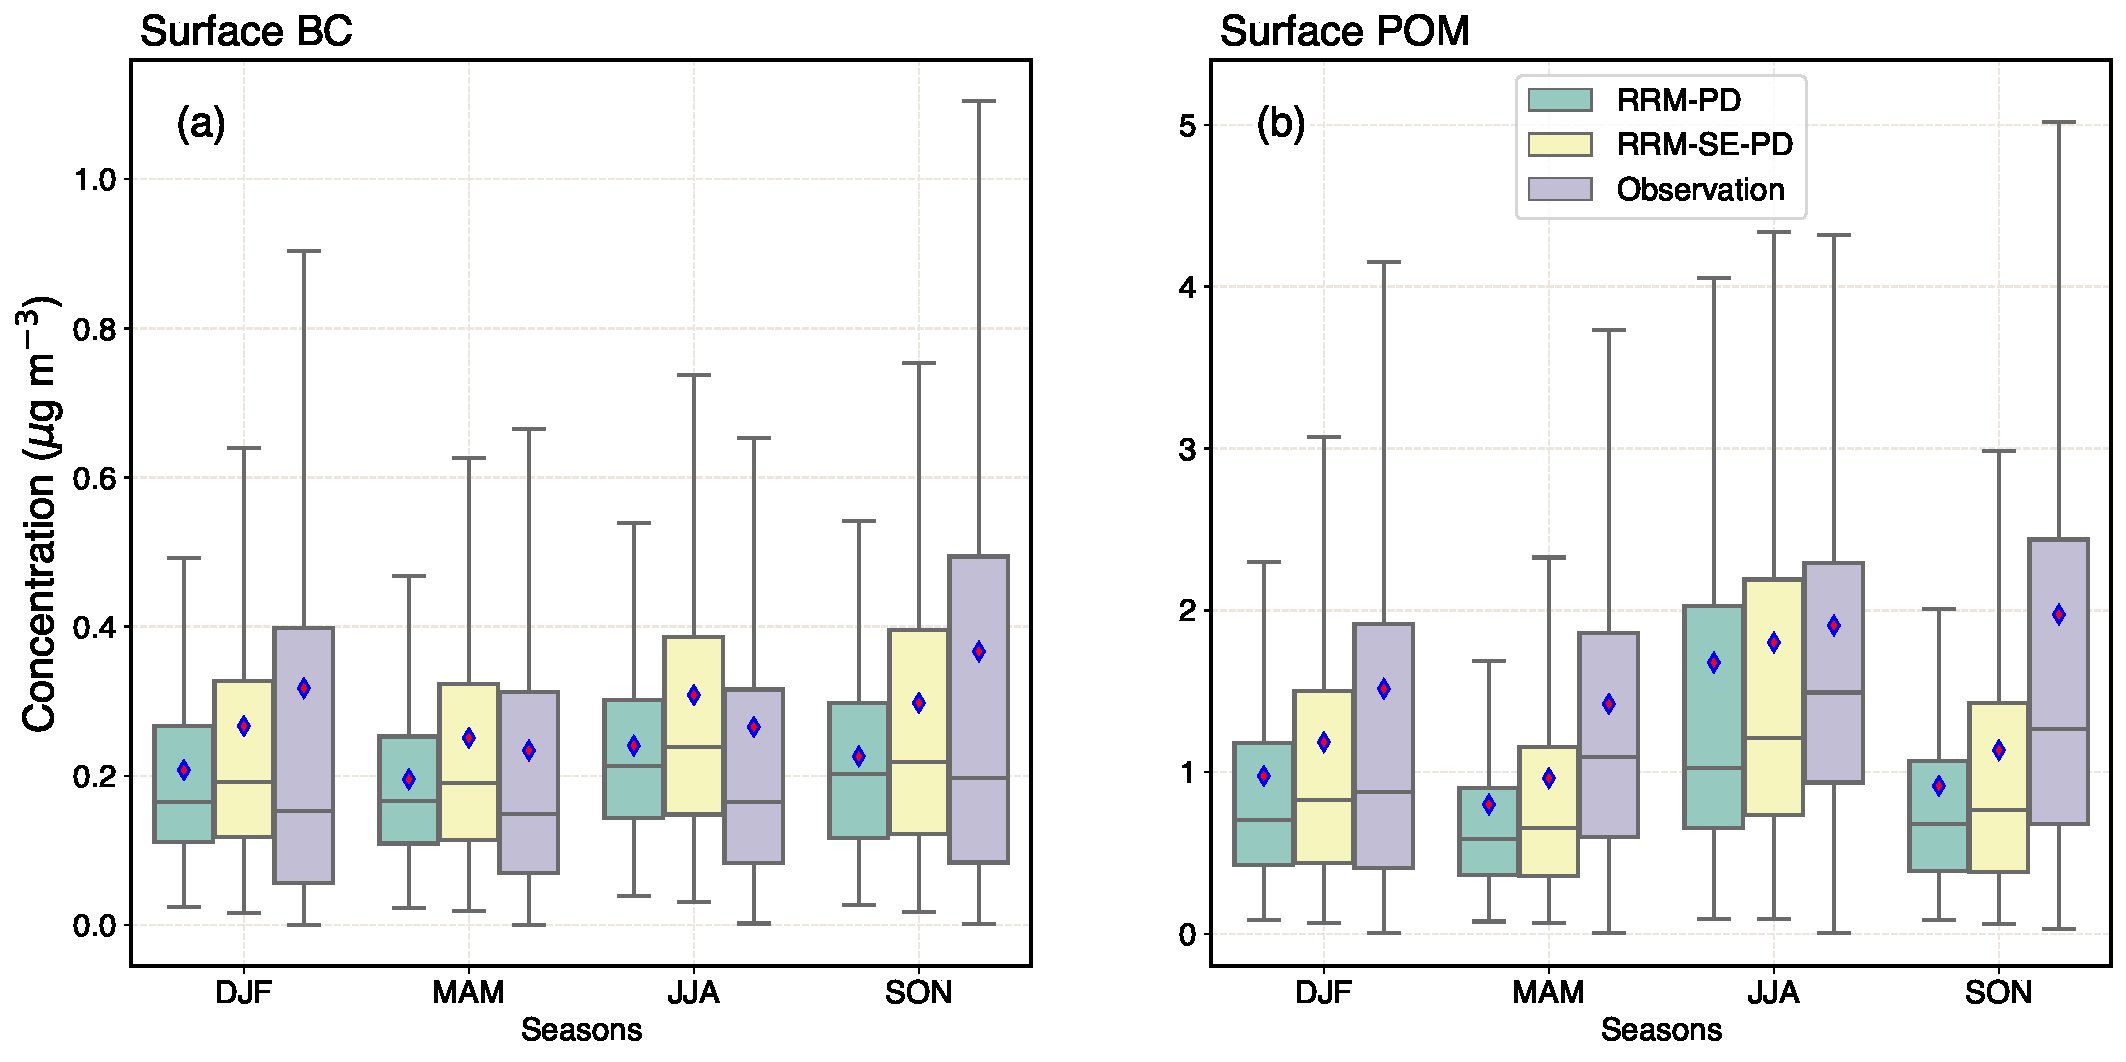
\includegraphics[width=16.5cm]{fig14.pdf}
\caption{Scatter plots between simulated and observed monthly mean surface concentrations of (a, c) sulfate (SO4) aerosols and (b, d) Aerosol Optical Depth (AOD) at 550 nm. Observations of the surface concentrations and AOD are from IMPROVE and AERONET respectively for the simulation year of 2016. Scatter plot statistics compare the spearman’s correlation (R), number of data points (n), RMSE, NMB values between (a, b) RRM-PD and (c, d) RRM-SE-PD simulation. RMSE and NMB are defined as in Table 2. Solid lines indicate the 1:1 ratio, and the dashed lines indicate the 1:2 and 2:1 ratio. The values at the top of each column indicate the observed mean.}
\end{figure}

%\begin{thebibliography}{}

%\bibitem[AUTHOR(YEAR)]{LABEL1}
%REFERENCE 1

%\bibitem[AUTHOR(YEAR)]{LABEL2}
%REFERENCE 2

%\end{thebibliography}

%% Since the Copernicus LaTeX package includes the BibTeX style file copernicus.bst,
%% authors experienced with BibTeX only have to include the following two lines:
%%
%% \bibliographystyle{copernicus}
%% \bibliography{example.bib}
%%
%% URLs and DOIs can be entered in your BibTeX file as:
%%
%% URL = {http://www.xyz.org/~jones/idx_g.htm}
%% DOI = {10.5194/xyz}


%% LITERATURE CITATIONS
%%
%% command                        & example result
%% \citet{jones90}|               & Jones et al. (1990)
%% \citep{jones90}|               & (Jones et al., 1990)
%% \citep{jones90,jones93}|       & (Jones et al., 1990, 1993)
%% \citep[p.~32]{jones90}|        & (Jones et al., 1990, p.~32)
%% \citep[e.g.,][]{jones90}|      & (e.g., Jones et al., 1990)
%% \citep[e.g.,][p.~32]{jones90}| & (e.g., Jones et al., 1990, p.~32)
%% \citeauthor{jones90}|          & Jones et al.
%% \citeyear{jones90}|            & 1990



%% FIGURES

%% When figures and tables are placed at the end of the MS (article in one-column style), please add \clearpage
%% between bibliography and first table and/or figure as well as between each table and/or figure.

% The figure files should be labelled correctly with Arabic numerals (e.g. fig01.jpg, fig02.png).


%% ONE-COLUMN FIGURES

%%f
%\begin{figure}[t]
%\includegraphics[width=8.3cm]{FILE NAME}
%\caption{TEXT}
%\end{figure}
%
%%% TWO-COLUMN FIGURES
%
%%f
%\begin{figure*}[t]
%\includegraphics[width=12cm]{FILE NAME}
%\caption{TEXT}
%\end{figure*}
%
%
%%% TABLES
%%%
%%% The different columns must be seperated with a & command and should
%%% end with \\ to identify the column brake.
%
%%% ONE-COLUMN TABLE
%
%%t
%\begin{table}[t]
%\caption{TEXT}
%\begin{tabular}{column = lcr}
%\tophline
%
%\middlehline
%
%\bottomhline
%\end{tabular}
%\belowtable{} % Table Footnotes
%\end{table}
%
%%% TWO-COLUMN TABLE
%
%%t
%\begin{table*}[t]
%\caption{TEXT}
%\begin{tabular}{column = lcr}
%\tophline
%
%\middlehline
%
%\bottomhline
%\end{tabular}
%\belowtable{} % Table Footnotes
%\end{table*}
%
%%% LANDSCAPE TABLE
%
%%t
%\begin{sidewaystable*}[t]
%\caption{TEXT}
%\begin{tabular}{column = lcr}
%\tophline
%
%\middlehline
%
%\bottomhline
%\end{tabular}
%\belowtable{} % Table Footnotes
%\end{sidewaystable*}
%
%
%%% MATHEMATICAL EXPRESSIONS
%
%%% All papers typeset by Copernicus Publications follow the math typesetting regulations
%%% given by the IUPAC Green Book (IUPAC: Quantities, Units and Symbols in Physical Chemistry,
%%% 2nd Edn., Blackwell Science, available at: http://old.iupac.org/publications/books/gbook/green_book_2ed.pdf, 1993).
%%%
%%% Physical quantities/variables are typeset in italic font (t for time, T for Temperature)
%%% Indices which are not defined are typeset in italic font (x, y, z, a, b, c)
%%% Items/objects which are defined are typeset in roman font (Car A, Car B)
%%% Descriptions/specifications which are defined by itself are typeset in roman font (abs, rel, ref, tot, net, ice)
%%% Abbreviations from 2 letters are typeset in roman font (RH, LAI)
%%% Vectors are identified in bold italic font using \vec{x}
%%% Matrices are identified in bold roman font
%%% Multiplication signs are typeset using the LaTeX commands \times (for vector products, grids, and exponential notations) or \cdot
%%% The character * should not be applied as mutliplication sign
%
%
%%% EQUATIONS
%
%%% Single-row equation
%
%\begin{equation}
%
%\end{equation}
%
%%% Multiline equation
%
%\begin{align}
%& 3 + 5 = 8\\
%& 3 + 5 = 8\\
%& 3 + 5 = 8
%\end{align}
%
%
%%% MATRICES
%
%\begin{matrix}
%x & y & z\\
%x & y & z\\
%x & y & z\\
%\end{matrix}
%
%
%%% ALGORITHM
%
%\begin{algorithm}
%\caption{...}
%\label{a1}
%\begin{algorithmic}
%...
%\end{algorithmic}
%\end{algorithm}
%
%
%%% CHEMICAL FORMULAS AND REACTIONS
%
%%% For formulas embedded in the text, please use \chem{}
%
%%% The reaction environment creates labels including the letter R, i.e. (R1), (R2), etc.
%
%\begin{reaction}
%%% \rightarrow should be used for normal (one-way) chemical reactions
%%% \rightleftharpoons should be used for equilibria
%%% \leftrightarrow should be used for resonance structures
%\end{reaction}
%
%
%%% PHYSICAL UNITS
%%%
%%% Please use \unit{} and apply the exponential notation


\end{document}
